% Seminarul 2: Distribuții clasice și fapte stilizate
% Statistica piețelor financiare -- Program de licență, Academia de Studii Economice din București
% GENERAT de latex/build_seminar2.py -- modificați generatorul, nu acest fișier.
% Implicit versiunea pentru studenți; versiunea profesorului este wrapper-ul *_solutions.tex.
\makeatletter\@ifundefined{ifsolutions}{\expandafter\newif\csname ifsolutions\endcsname}{}\makeatother

\newcommand{\coursename}{Statistica piețelor financiare}
\def\sfmlang{ro}
% Preambul comun SFM -- Statistica piețelor financiare / Statistics of Financial Markets (Beamer, 16:9)
% Același design ca MFM. Înainte de % Preambul comun SFM -- Statistica piețelor financiare / Statistics of Financial Markets (Beamer, 16:9)
% Același design ca MFM. Înainte de % Preambul comun SFM -- Statistica piețelor financiare / Statistics of Financial Markets (Beamer, 16:9)
% Același design ca MFM. Înainte de \input{../../latex/preamble} se definește
%   \newcommand{\coursename}{Statistics of Financial Markets}      (EN)
%   \newcommand{\coursename}{Statistica piețelor financiare}       (RO)  și  \def\sfmlang{ro}
% Fișierele .tex se află în EN/Courses, EN/Seminars, RO/Cursuri, RO/Seminarii (două niveluri sub rădăcină).
% Deck-urile sînt generate de latex/build_chapterN.py / build_seminarN.py (vezi latex/sfm_build.py).

\documentclass[9pt, aspectratio=169, t]{beamer}
\providecommand{\coursename}{Statistics of Financial Markets}

% Ensure content fits on slides
\setbeamersize{text margin left=8mm, text margin right=8mm}

%=============================================================================
% THEME AND STYLE CONFIGURATION
%=============================================================================
\usetheme{default}
% Using default theme for clean header/footer control

% Color Palette (matching Redispatch PDF)
\definecolor{MainBlue}{RGB}{26, 58, 110}
\definecolor{AccentBlue}{RGB}{26, 58, 110}
\definecolor{IDAred}{RGB}{205, 0, 0}
\definecolor{DarkGray}{RGB}{51, 51, 51}
\definecolor{MediumGray}{RGB}{128, 128, 128}
\definecolor{LightGray}{RGB}{248, 248, 248}
\definecolor{VeryLightGray}{RGB}{235, 235, 235}
\definecolor{KeynoteGray}{RGB}{218, 218, 218}
\definecolor{SectionGray}{RGB}{120, 120, 120}
\definecolor{FooterGray}{RGB}{100, 100, 100}
\definecolor{Crimson}{RGB}{220, 53, 69}
\definecolor{Forest}{RGB}{46, 125, 50}
\definecolor{Amber}{RGB}{181, 133, 63}
\definecolor{Orange}{RGB}{230, 126, 34}
\definecolor{Purple}{RGB}{142, 68, 173}

% Gradient background (exact Keynote 315° gradient: white to RGB 218,218,218)
\setbeamertemplate{background}{%
    \begin{tikzpicture}[remember picture, overlay]
        \shade[shading=axis, shading angle=315,
        top color=white, bottom color=KeynoteGray]
        (current page.south west) rectangle (current page.north east);
    \end{tikzpicture}%
}
% Fallback solid color for compatibility
\setbeamercolor{background canvas}{bg=}

\setbeamercolor{palette primary}{bg=MainBlue, fg=white}
\setbeamercolor{palette secondary}{bg=MainBlue!85, fg=white}
\setbeamercolor{palette tertiary}{bg=MainBlue!70, fg=white}
\setbeamercolor{structure}{fg=MainBlue}
\setbeamercolor{title}{fg=IDAred}
\setbeamercolor{frametitle}{fg=IDAred, bg=}
\setbeamercolor{block title}{bg=MainBlue, fg=white}
\setbeamercolor{block body}{bg=VeryLightGray, fg=DarkGray}
\setbeamercolor{block title alerted}{bg=Crimson, fg=white}
\setbeamercolor{block body alerted}{bg=Crimson!8, fg=DarkGray}
\setbeamercolor{block title example}{bg=Forest, fg=white}
\setbeamercolor{block body example}{bg=Forest!8, fg=DarkGray}
\setbeamercolor{item}{fg=MainBlue}

% Footer colors (override Madrid theme blue)
\setbeamercolor{author in head/foot}{fg=FooterGray, bg=}
\setbeamercolor{title in head/foot}{fg=FooterGray, bg=}
\setbeamercolor{date in head/foot}{fg=FooterGray, bg=}
\setbeamercolor{section in head/foot}{fg=FooterGray, bg=}
\setbeamercolor{subsection in head/foot}{fg=FooterGray, bg=}

% Bullet styles (apply everywhere including blocks)
\setbeamertemplate{itemize item}{\color{MainBlue}$\boxdot$}
\setbeamertemplate{itemize subitem}{\color{MainBlue}$\blacktriangleright$}
\setbeamertemplate{itemize subsubitem}{\color{MainBlue}\tiny$\bullet$}
\setbeamertemplate{itemize/enumerate body begin}{\normalsize}
\setbeamertemplate{itemize/enumerate subbody begin}{\normalsize}

% Item spacing - compact style
\setlength{\leftmargini}{10pt}       % Level 1: minimal indent
\setlength{\leftmarginii}{10pt}      % Level 2: minimal additional indent
% Compact list spacing (zero extra space before/after lists in blocks)
\makeatletter
\def\@listi{\leftmargin\leftmargini \topsep 0pt \parsep 0pt \itemsep 0pt}
\def\@listii{\leftmargin\leftmarginii \topsep 0pt \parsep 0pt \itemsep 0pt}
\makeatother

\setbeamertemplate{navigation symbols}{}

%=============================================================================
% CUSTOM HEADLINE
%=============================================================================
\setbeamertemplate{headline}{%
    \vskip10pt%
    \hbox to \paperwidth{%
        \hskip0.5cm%
        {\small\color{FooterGray}\renewcommand{\hyperlink}[2]{##2}\insertsectionhead}%
        \hfill%
        \textcolor{FooterGray}{\small\insertframenumber}%
        \hskip0.5cm%
    }%
    \vskip4pt%
    {\color{FooterGray}\hrule height 0.4pt}%
}

%=============================================================================
% CUSTOM FOOTER
%=============================================================================
\usepackage{fontawesome5}

\setbeamertemplate{footline}{%
    {\color{FooterGray}\hrule height 0.4pt}%
    \vskip4pt%
    \hbox to \paperwidth{%
        \hskip0.5cm%
        \textcolor{FooterGray}{\small\coursename}%
        \hfill%
        \raisebox{-0.1em}{%
            \begin{tikzpicture}[x=0.08em, y=0.08em, line width=0.4pt]
                \draw[FooterGray] (0,3) -- (1,4) -- (2,3.5) -- (3,5) -- (4,4) -- (5,6) -- (6,5.5) -- (7,4) -- (8,5) -- (9,7) -- (10,6) -- (11,5) -- (12,6.5) -- (13,8) -- (14,7) -- (15,6) -- (16,7.5) -- (17,9) -- (18,8) -- (19,7) -- (20,8.5) -- (21,10) -- (22,9) -- (23,8) -- (24,9.5);
            \end{tikzpicture}%
        }%
        \hskip0.5cm%
    }%
    \vskip6pt%
}

%=============================================================================
% PACKAGES
%=============================================================================
\usepackage[utf8]{inputenc}
\DeclareUnicodeCharacter{03B1}{\ensuremath{\alpha}}
\usepackage[T1]{fontenc}
\usepackage{amsmath, amssymb, amsthm}
\usepackage{mathtools}
\usepackage{bm}
\usepackage{tikz}
\usetikzlibrary{arrows.meta, positioning, shapes, calc, decorations.pathreplacing, shadings}
\usepackage{booktabs}
\usepackage{multirow}
\usepackage{array}
\usepackage{graphicx}
\usepackage{hyperref}
\usepackage{colortbl}
\usepackage{listings}
\lstset{language=Python, basicstyle=\ttfamily\scriptsize, keywordstyle=\color{MainBlue}\bfseries,
  commentstyle=\color{Forest}, stringstyle=\color{Crimson}, breaklines=true,
  frame=none, backgroundcolor=\color{VeryLightGray}, xleftmargin=2mm}
\hypersetup{colorlinks=true, linkcolor=MainBlue, urlcolor=MainBlue}
\graphicspath{{../../logos/}{../../charts/}{../../photos/}}
\usepackage{xcolor}
\hfuzz=2pt  % Suppress tiny overfull warnings (<2pt)
\vfuzz=2pt  % Suppress tiny vertical overfull warnings (<2pt)

%=============================================================================
% QUANTLET COMMANDS
%   \quantlet{<displayed name>}{<url>}       (generic, compatible with the older SFM decks)
%   \sfmquantlet{Ch_05}{SFM_ch5_garch}       -> https://github.com/danpele/SFM/tree/main/Quantlets/Ch_05/SFM_ch5_garch
%   \qlurl{<folder>} is defined per chapter by the generator (Quantlets/Ch_NN/<folder>)
%=============================================================================
\newcommand{\sfmrepo}{https://github.com/danpele/SFM}
\newcommand{\sfmqlbase}{https://github.com/danpele/SFM/tree/main/Quantlets}
\newcommand{\quantlet}[2]{%
    \hfill\href{#2}{%
        \raisebox{-0.15em}{
\includegraphics[height=0.7em]{ql_logo.png}}%
        \textcolor{MainBlue}{\tiny\ #1}%
    }%
}
\newcommand{\sfmquantlet}[2]{\quantlet{\detokenize{#2}}{\sfmqlbase/#1/#2}}

%=============================================================================
% NOTEBOOKS (Google Colab)
%   \colaburl{notebooks/EN/chapter5_seminar_notebook.ipynb} -> the Colab link of a file in the SFM repo
%   \nb: the chapter notebook (each seminar deck redefines it with \renewcommand)
%=============================================================================
\newcommand{\colaburl}[1]{https://colab.research.google.com/github/danpele/SFM/blob/main/#1}
\newcommand{\nb}{https://colab.research.google.com/github/danpele/SFM/tree/main/notebooks/EN}
\newcommand{\nbname}{notebooks/EN}

%=============================================================================
% SLIDE HELPERS (used by the generators; the same as in MFM)
%=============================================================================
% local font size for list bodies (the preamble forces \normalsize)
\newcommand{\itemsize}[1]{\setbeamertemplate{itemize/enumerate body begin}{#1}\setbeamertemplate{itemize/enumerate subbody begin}{#1}}
\newcommand{\intitle}[1]{{\hypersetup{urlcolor=white}#1}}   % white links inside coloured title bars
\newcommand{\imgcap}[1]{{\scriptsize #1}\\[0.5mm]}          % caption under a photo
\newcommand{\imgcredit}[2]{{\tiny\color{FooterGray}\href{#1}{#2}}}   % image credit: source URL, author/licence
\newcommand{\aiprompt}[1]{{\ttfamily\color{MainBlue}#1}}     % a prompt to an AI assistant

%=============================================================================
% SEMINARS: student version by default; the instructor wrapper *_solutions.tex sets \solutionstrue
%=============================================================================
\makeatletter\@ifundefined{ifsolutions}{\expandafter\newif\csname ifsolutions\endcsname}{}\makeatother
\newcommand{\solonly}[1]{\ifsolutions #1\fi}
\newcommand{\propsub}{\ifsolutions\else\framesubtitle{\ifdefined\sfmlang Rezolvarea se discută la seminar\else Solution discussed in class\fi}\fi}

%=============================================================================
% APPENDIX AND CHAPTER LINKS (latex/appendix_links.py writes the calls; it also re-declares these
% macros before \begin{document}, so the decks compile with or without this preamble block)
%=============================================================================
\providecommand{\sfmapplink}[3]{\hypertarget{#2}{}\hyperlink{#1}{\beamergotobutton{#3}}}
\providecommand{\sfmappback}[2]{\begin{tikzpicture}[remember picture,overlay]\node[anchor=south east] at ([xshift=-3mm,yshift=7mm]current page.south east){\hyperlink{#1}{\beamerreturnbutton{#2}}};\end{tikzpicture}}
\providecommand{\sfmchlink}[2]{\href{#1}{#2}}
\providecommand{\sfmchlinkt}[2]{\href{#1}{\usebeamercolor[fg]{frametitle}#2}}

%=============================================================================
% QUANTINAR COMMAND: link către un curs Quantinar (subiecte avansate)
%=============================================================================
\newcommand{\quantinar}[2]{%
    \href{#2}{%
        \raisebox{-0.15em}{
\includegraphics[height=0.8em]{qr_logo.png}}%
        \textcolor{MainBlue}{\scriptsize\ #1}%
    }%
}

%=============================================================================
% CUSTOM TITLE PAGE
%=============================================================================
\defbeamertemplate*{title page}{hybrid}[1][]
{
    \vspace{0.2cm}
    % Logos row - top header (with clickable links)
    \begin{center}
        \href{https://www.ase.ro}{
\includegraphics[height=1.0cm]{ase_logo.png}}\hspace{0.3cm}%
        \href{https://theida.net}{
\includegraphics[height=1.0cm]{ida_logo.png}}\hspace{0.3cm}%
        \href{https://blockchain-research-center.com}{
\includegraphics[height=1.0cm]{brc_logo.png}}\hspace{0.3cm}%
        \href{https://www.ai4efin.ase.ro}{
\includegraphics[height=1.0cm]{ai4efin_logo.png}}\hspace{0.3cm}%
        \href{https://ipe.ro/new}{
\includegraphics[height=1.0cm]{acad_logo.png}}\hspace{0.3cm}%
        \href{https://www.digital-finance-msca.com}{
\includegraphics[height=1.0cm]{msca_logo.png}}%
    \end{center}

    \vspace{0.6cm}

    % Main title with Q logos on sides (with clickable links)
    \begin{center}
        \begin{minipage}{0.1\textwidth}
            \centering
            \href{https://quantlet.com}{
\includegraphics[height=1.1cm]{ql_logo.png}}
        \end{minipage}%
        \begin{minipage}{0.78\textwidth}
            \centering
            {\LARGE\bfseries\usebeamercolor[fg]{title}\inserttitle}

            \vspace{0.3cm}

            {\usebeamerfont{subtitle}\usebeamercolor[fg]{title}\insertsubtitle}
        \end{minipage}%
        \begin{minipage}{0.1\textwidth}
            \centering
            \href{https://quantinar.com}{
\includegraphics[height=1.1cm]{qr_logo.png}}
        \end{minipage}
    \end{center}

    \vspace{0.6cm}

    % Authors (left aligned)
    \hspace{0.5cm}{\usebeamerfont{author}\insertauthor}

    \vspace{0.3cm}

    % Institute/Affiliations (left aligned)
    \hspace{0.5cm}\begin{minipage}[t]{0.9\textwidth}
        \raggedright\small\insertinstitute
    \end{minipage}
}

%=============================================================================
% THEOREM ENVIRONMENTS
%=============================================================================
\theoremstyle{definition}
\setbeamertemplate{theorems}[numbered]
\ifdefined\sfmlang
\newtheorem{defn}{Definiție}
\newtheorem{thm}{Teoremă}
\newtheorem{prop}{Propoziție}
\newtheorem{rmk}{Observație}
\else
\newtheorem{defn}{Definition}
\newtheorem{thm}{Theorem}
\newtheorem{prop}{Proposition}
\newtheorem{rmk}{Remark}
\fi

%=============================================================================
% CENTRED MINIPAGE (no extra vertical space)
%=============================================================================
\newenvironment{cminipage}[1]{%
    \par\noindent\hfill\begin{minipage}{#1}\ignorespaces
}{%
    \end{minipage}\hfill\null\par
}

%=============================================================================
% CUSTOM COMMANDS
%=============================================================================
\newcommand{\E}{\mathbb{E}}
\newcommand{\Var}{\text{Var}}
\newcommand{\Cov}{\text{Cov}}
\newcommand{\Corr}{\text{Corr}}
\newcommand{\R}{\mathbb{R}}
\newcommand{\N}{\mathbb{N}}
\newcommand{\Z}{\mathbb{Z}}
\newcommand{\B}{\mathbf{B}}
\newcommand{\imark}{\textcolor{MainBlue}{\textbullet}}
\newcommand{\RMSE}{\text{RMSE}}
\newcommand{\MAE}{\text{MAE}}
\newcommand{\MAPE}{\text{MAPE}}

 se definește
%   \newcommand{\coursename}{Statistics of Financial Markets}      (EN)
%   \newcommand{\coursename}{Statistica piețelor financiare}       (RO)  și  \def\sfmlang{ro}
% Fișierele .tex se află în EN/Courses, EN/Seminars, RO/Cursuri, RO/Seminarii (două niveluri sub rădăcină).
% Deck-urile sînt generate de latex/build_chapterN.py / build_seminarN.py (vezi latex/sfm_build.py).

\documentclass[9pt, aspectratio=169, t]{beamer}
\providecommand{\coursename}{Statistics of Financial Markets}

% Ensure content fits on slides
\setbeamersize{text margin left=8mm, text margin right=8mm}

%=============================================================================
% THEME AND STYLE CONFIGURATION
%=============================================================================
\usetheme{default}
% Using default theme for clean header/footer control

% Color Palette (matching Redispatch PDF)
\definecolor{MainBlue}{RGB}{26, 58, 110}
\definecolor{AccentBlue}{RGB}{26, 58, 110}
\definecolor{IDAred}{RGB}{205, 0, 0}
\definecolor{DarkGray}{RGB}{51, 51, 51}
\definecolor{MediumGray}{RGB}{128, 128, 128}
\definecolor{LightGray}{RGB}{248, 248, 248}
\definecolor{VeryLightGray}{RGB}{235, 235, 235}
\definecolor{KeynoteGray}{RGB}{218, 218, 218}
\definecolor{SectionGray}{RGB}{120, 120, 120}
\definecolor{FooterGray}{RGB}{100, 100, 100}
\definecolor{Crimson}{RGB}{220, 53, 69}
\definecolor{Forest}{RGB}{46, 125, 50}
\definecolor{Amber}{RGB}{181, 133, 63}
\definecolor{Orange}{RGB}{230, 126, 34}
\definecolor{Purple}{RGB}{142, 68, 173}

% Gradient background (exact Keynote 315° gradient: white to RGB 218,218,218)
\setbeamertemplate{background}{%
    \begin{tikzpicture}[remember picture, overlay]
        \shade[shading=axis, shading angle=315,
        top color=white, bottom color=KeynoteGray]
        (current page.south west) rectangle (current page.north east);
    \end{tikzpicture}%
}
% Fallback solid color for compatibility
\setbeamercolor{background canvas}{bg=}

\setbeamercolor{palette primary}{bg=MainBlue, fg=white}
\setbeamercolor{palette secondary}{bg=MainBlue!85, fg=white}
\setbeamercolor{palette tertiary}{bg=MainBlue!70, fg=white}
\setbeamercolor{structure}{fg=MainBlue}
\setbeamercolor{title}{fg=IDAred}
\setbeamercolor{frametitle}{fg=IDAred, bg=}
\setbeamercolor{block title}{bg=MainBlue, fg=white}
\setbeamercolor{block body}{bg=VeryLightGray, fg=DarkGray}
\setbeamercolor{block title alerted}{bg=Crimson, fg=white}
\setbeamercolor{block body alerted}{bg=Crimson!8, fg=DarkGray}
\setbeamercolor{block title example}{bg=Forest, fg=white}
\setbeamercolor{block body example}{bg=Forest!8, fg=DarkGray}
\setbeamercolor{item}{fg=MainBlue}

% Footer colors (override Madrid theme blue)
\setbeamercolor{author in head/foot}{fg=FooterGray, bg=}
\setbeamercolor{title in head/foot}{fg=FooterGray, bg=}
\setbeamercolor{date in head/foot}{fg=FooterGray, bg=}
\setbeamercolor{section in head/foot}{fg=FooterGray, bg=}
\setbeamercolor{subsection in head/foot}{fg=FooterGray, bg=}

% Bullet styles (apply everywhere including blocks)
\setbeamertemplate{itemize item}{\color{MainBlue}$\boxdot$}
\setbeamertemplate{itemize subitem}{\color{MainBlue}$\blacktriangleright$}
\setbeamertemplate{itemize subsubitem}{\color{MainBlue}\tiny$\bullet$}
\setbeamertemplate{itemize/enumerate body begin}{\normalsize}
\setbeamertemplate{itemize/enumerate subbody begin}{\normalsize}

% Item spacing - compact style
\setlength{\leftmargini}{10pt}       % Level 1: minimal indent
\setlength{\leftmarginii}{10pt}      % Level 2: minimal additional indent
% Compact list spacing (zero extra space before/after lists in blocks)
\makeatletter
\def\@listi{\leftmargin\leftmargini \topsep 0pt \parsep 0pt \itemsep 0pt}
\def\@listii{\leftmargin\leftmarginii \topsep 0pt \parsep 0pt \itemsep 0pt}
\makeatother

\setbeamertemplate{navigation symbols}{}

%=============================================================================
% CUSTOM HEADLINE
%=============================================================================
\setbeamertemplate{headline}{%
    \vskip10pt%
    \hbox to \paperwidth{%
        \hskip0.5cm%
        {\small\color{FooterGray}\renewcommand{\hyperlink}[2]{##2}\insertsectionhead}%
        \hfill%
        \textcolor{FooterGray}{\small\insertframenumber}%
        \hskip0.5cm%
    }%
    \vskip4pt%
    {\color{FooterGray}\hrule height 0.4pt}%
}

%=============================================================================
% CUSTOM FOOTER
%=============================================================================
\usepackage{fontawesome5}

\setbeamertemplate{footline}{%
    {\color{FooterGray}\hrule height 0.4pt}%
    \vskip4pt%
    \hbox to \paperwidth{%
        \hskip0.5cm%
        \textcolor{FooterGray}{\small\coursename}%
        \hfill%
        \raisebox{-0.1em}{%
            \begin{tikzpicture}[x=0.08em, y=0.08em, line width=0.4pt]
                \draw[FooterGray] (0,3) -- (1,4) -- (2,3.5) -- (3,5) -- (4,4) -- (5,6) -- (6,5.5) -- (7,4) -- (8,5) -- (9,7) -- (10,6) -- (11,5) -- (12,6.5) -- (13,8) -- (14,7) -- (15,6) -- (16,7.5) -- (17,9) -- (18,8) -- (19,7) -- (20,8.5) -- (21,10) -- (22,9) -- (23,8) -- (24,9.5);
            \end{tikzpicture}%
        }%
        \hskip0.5cm%
    }%
    \vskip6pt%
}

%=============================================================================
% PACKAGES
%=============================================================================
\usepackage[utf8]{inputenc}
\DeclareUnicodeCharacter{03B1}{\ensuremath{\alpha}}
\usepackage[T1]{fontenc}
\usepackage{amsmath, amssymb, amsthm}
\usepackage{mathtools}
\usepackage{bm}
\usepackage{tikz}
\usetikzlibrary{arrows.meta, positioning, shapes, calc, decorations.pathreplacing, shadings}
\usepackage{booktabs}
\usepackage{multirow}
\usepackage{array}
\usepackage{graphicx}
\usepackage{hyperref}
\usepackage{colortbl}
\usepackage{listings}
\lstset{language=Python, basicstyle=\ttfamily\scriptsize, keywordstyle=\color{MainBlue}\bfseries,
  commentstyle=\color{Forest}, stringstyle=\color{Crimson}, breaklines=true,
  frame=none, backgroundcolor=\color{VeryLightGray}, xleftmargin=2mm}
\hypersetup{colorlinks=true, linkcolor=MainBlue, urlcolor=MainBlue}
\graphicspath{{../../logos/}{../../charts/}{../../photos/}}
\usepackage{xcolor}
\hfuzz=2pt  % Suppress tiny overfull warnings (<2pt)
\vfuzz=2pt  % Suppress tiny vertical overfull warnings (<2pt)

%=============================================================================
% QUANTLET COMMANDS
%   \quantlet{<displayed name>}{<url>}       (generic, compatible with the older SFM decks)
%   \sfmquantlet{Ch_05}{SFM_ch5_garch}       -> https://github.com/danpele/SFM/tree/main/Quantlets/Ch_05/SFM_ch5_garch
%   \qlurl{<folder>} is defined per chapter by the generator (Quantlets/Ch_NN/<folder>)
%=============================================================================
\newcommand{\sfmrepo}{https://github.com/danpele/SFM}
\newcommand{\sfmqlbase}{https://github.com/danpele/SFM/tree/main/Quantlets}
\newcommand{\quantlet}[2]{%
    \hfill\href{#2}{%
        \raisebox{-0.15em}{
\includegraphics[height=0.7em]{ql_logo.png}}%
        \textcolor{MainBlue}{\tiny\ #1}%
    }%
}
\newcommand{\sfmquantlet}[2]{\quantlet{\detokenize{#2}}{\sfmqlbase/#1/#2}}

%=============================================================================
% NOTEBOOKS (Google Colab)
%   \colaburl{notebooks/EN/chapter5_seminar_notebook.ipynb} -> the Colab link of a file in the SFM repo
%   \nb: the chapter notebook (each seminar deck redefines it with \renewcommand)
%=============================================================================
\newcommand{\colaburl}[1]{https://colab.research.google.com/github/danpele/SFM/blob/main/#1}
\newcommand{\nb}{https://colab.research.google.com/github/danpele/SFM/tree/main/notebooks/EN}
\newcommand{\nbname}{notebooks/EN}

%=============================================================================
% SLIDE HELPERS (used by the generators; the same as in MFM)
%=============================================================================
% local font size for list bodies (the preamble forces \normalsize)
\newcommand{\itemsize}[1]{\setbeamertemplate{itemize/enumerate body begin}{#1}\setbeamertemplate{itemize/enumerate subbody begin}{#1}}
\newcommand{\intitle}[1]{{\hypersetup{urlcolor=white}#1}}   % white links inside coloured title bars
\newcommand{\imgcap}[1]{{\scriptsize #1}\\[0.5mm]}          % caption under a photo
\newcommand{\imgcredit}[2]{{\tiny\color{FooterGray}\href{#1}{#2}}}   % image credit: source URL, author/licence
\newcommand{\aiprompt}[1]{{\ttfamily\color{MainBlue}#1}}     % a prompt to an AI assistant

%=============================================================================
% SEMINARS: student version by default; the instructor wrapper *_solutions.tex sets \solutionstrue
%=============================================================================
\makeatletter\@ifundefined{ifsolutions}{\expandafter\newif\csname ifsolutions\endcsname}{}\makeatother
\newcommand{\solonly}[1]{\ifsolutions #1\fi}
\newcommand{\propsub}{\ifsolutions\else\framesubtitle{\ifdefined\sfmlang Rezolvarea se discută la seminar\else Solution discussed in class\fi}\fi}

%=============================================================================
% APPENDIX AND CHAPTER LINKS (latex/appendix_links.py writes the calls; it also re-declares these
% macros before \begin{document}, so the decks compile with or without this preamble block)
%=============================================================================
\providecommand{\sfmapplink}[3]{\hypertarget{#2}{}\hyperlink{#1}{\beamergotobutton{#3}}}
\providecommand{\sfmappback}[2]{\begin{tikzpicture}[remember picture,overlay]\node[anchor=south east] at ([xshift=-3mm,yshift=7mm]current page.south east){\hyperlink{#1}{\beamerreturnbutton{#2}}};\end{tikzpicture}}
\providecommand{\sfmchlink}[2]{\href{#1}{#2}}
\providecommand{\sfmchlinkt}[2]{\href{#1}{\usebeamercolor[fg]{frametitle}#2}}

%=============================================================================
% QUANTINAR COMMAND: link către un curs Quantinar (subiecte avansate)
%=============================================================================
\newcommand{\quantinar}[2]{%
    \href{#2}{%
        \raisebox{-0.15em}{
\includegraphics[height=0.8em]{qr_logo.png}}%
        \textcolor{MainBlue}{\scriptsize\ #1}%
    }%
}

%=============================================================================
% CUSTOM TITLE PAGE
%=============================================================================
\defbeamertemplate*{title page}{hybrid}[1][]
{
    \vspace{0.2cm}
    % Logos row - top header (with clickable links)
    \begin{center}
        \href{https://www.ase.ro}{
\includegraphics[height=1.0cm]{ase_logo.png}}\hspace{0.3cm}%
        \href{https://theida.net}{
\includegraphics[height=1.0cm]{ida_logo.png}}\hspace{0.3cm}%
        \href{https://blockchain-research-center.com}{
\includegraphics[height=1.0cm]{brc_logo.png}}\hspace{0.3cm}%
        \href{https://www.ai4efin.ase.ro}{
\includegraphics[height=1.0cm]{ai4efin_logo.png}}\hspace{0.3cm}%
        \href{https://ipe.ro/new}{
\includegraphics[height=1.0cm]{acad_logo.png}}\hspace{0.3cm}%
        \href{https://www.digital-finance-msca.com}{
\includegraphics[height=1.0cm]{msca_logo.png}}%
    \end{center}

    \vspace{0.6cm}

    % Main title with Q logos on sides (with clickable links)
    \begin{center}
        \begin{minipage}{0.1\textwidth}
            \centering
            \href{https://quantlet.com}{
\includegraphics[height=1.1cm]{ql_logo.png}}
        \end{minipage}%
        \begin{minipage}{0.78\textwidth}
            \centering
            {\LARGE\bfseries\usebeamercolor[fg]{title}\inserttitle}

            \vspace{0.3cm}

            {\usebeamerfont{subtitle}\usebeamercolor[fg]{title}\insertsubtitle}
        \end{minipage}%
        \begin{minipage}{0.1\textwidth}
            \centering
            \href{https://quantinar.com}{
\includegraphics[height=1.1cm]{qr_logo.png}}
        \end{minipage}
    \end{center}

    \vspace{0.6cm}

    % Authors (left aligned)
    \hspace{0.5cm}{\usebeamerfont{author}\insertauthor}

    \vspace{0.3cm}

    % Institute/Affiliations (left aligned)
    \hspace{0.5cm}\begin{minipage}[t]{0.9\textwidth}
        \raggedright\small\insertinstitute
    \end{minipage}
}

%=============================================================================
% THEOREM ENVIRONMENTS
%=============================================================================
\theoremstyle{definition}
\setbeamertemplate{theorems}[numbered]
\ifdefined\sfmlang
\newtheorem{defn}{Definiție}
\newtheorem{thm}{Teoremă}
\newtheorem{prop}{Propoziție}
\newtheorem{rmk}{Observație}
\else
\newtheorem{defn}{Definition}
\newtheorem{thm}{Theorem}
\newtheorem{prop}{Proposition}
\newtheorem{rmk}{Remark}
\fi

%=============================================================================
% CENTRED MINIPAGE (no extra vertical space)
%=============================================================================
\newenvironment{cminipage}[1]{%
    \par\noindent\hfill\begin{minipage}{#1}\ignorespaces
}{%
    \end{minipage}\hfill\null\par
}

%=============================================================================
% CUSTOM COMMANDS
%=============================================================================
\newcommand{\E}{\mathbb{E}}
\newcommand{\Var}{\text{Var}}
\newcommand{\Cov}{\text{Cov}}
\newcommand{\Corr}{\text{Corr}}
\newcommand{\R}{\mathbb{R}}
\newcommand{\N}{\mathbb{N}}
\newcommand{\Z}{\mathbb{Z}}
\newcommand{\B}{\mathbf{B}}
\newcommand{\imark}{\textcolor{MainBlue}{\textbullet}}
\newcommand{\RMSE}{\text{RMSE}}
\newcommand{\MAE}{\text{MAE}}
\newcommand{\MAPE}{\text{MAPE}}

 se definește
%   \newcommand{\coursename}{Statistics of Financial Markets}      (EN)
%   \newcommand{\coursename}{Statistica piețelor financiare}       (RO)  și  \def\sfmlang{ro}
% Fișierele .tex se află în EN/Courses, EN/Seminars, RO/Cursuri, RO/Seminarii (două niveluri sub rădăcină).
% Deck-urile sînt generate de latex/build_chapterN.py / build_seminarN.py (vezi latex/sfm_build.py).

\documentclass[9pt, aspectratio=169, t]{beamer}
\providecommand{\coursename}{Statistics of Financial Markets}

% Ensure content fits on slides
\setbeamersize{text margin left=8mm, text margin right=8mm}

%=============================================================================
% THEME AND STYLE CONFIGURATION
%=============================================================================
\usetheme{default}
% Using default theme for clean header/footer control

% Color Palette (matching Redispatch PDF)
\definecolor{MainBlue}{RGB}{26, 58, 110}
\definecolor{AccentBlue}{RGB}{26, 58, 110}
\definecolor{IDAred}{RGB}{205, 0, 0}
\definecolor{DarkGray}{RGB}{51, 51, 51}
\definecolor{MediumGray}{RGB}{128, 128, 128}
\definecolor{LightGray}{RGB}{248, 248, 248}
\definecolor{VeryLightGray}{RGB}{235, 235, 235}
\definecolor{KeynoteGray}{RGB}{218, 218, 218}
\definecolor{SectionGray}{RGB}{120, 120, 120}
\definecolor{FooterGray}{RGB}{100, 100, 100}
\definecolor{Crimson}{RGB}{220, 53, 69}
\definecolor{Forest}{RGB}{46, 125, 50}
\definecolor{Amber}{RGB}{181, 133, 63}
\definecolor{Orange}{RGB}{230, 126, 34}
\definecolor{Purple}{RGB}{142, 68, 173}

% Gradient background (exact Keynote 315° gradient: white to RGB 218,218,218)
\setbeamertemplate{background}{%
    \begin{tikzpicture}[remember picture, overlay]
        \shade[shading=axis, shading angle=315,
        top color=white, bottom color=KeynoteGray]
        (current page.south west) rectangle (current page.north east);
    \end{tikzpicture}%
}
% Fallback solid color for compatibility
\setbeamercolor{background canvas}{bg=}

\setbeamercolor{palette primary}{bg=MainBlue, fg=white}
\setbeamercolor{palette secondary}{bg=MainBlue!85, fg=white}
\setbeamercolor{palette tertiary}{bg=MainBlue!70, fg=white}
\setbeamercolor{structure}{fg=MainBlue}
\setbeamercolor{title}{fg=IDAred}
\setbeamercolor{frametitle}{fg=IDAred, bg=}
\setbeamercolor{block title}{bg=MainBlue, fg=white}
\setbeamercolor{block body}{bg=VeryLightGray, fg=DarkGray}
\setbeamercolor{block title alerted}{bg=Crimson, fg=white}
\setbeamercolor{block body alerted}{bg=Crimson!8, fg=DarkGray}
\setbeamercolor{block title example}{bg=Forest, fg=white}
\setbeamercolor{block body example}{bg=Forest!8, fg=DarkGray}
\setbeamercolor{item}{fg=MainBlue}

% Footer colors (override Madrid theme blue)
\setbeamercolor{author in head/foot}{fg=FooterGray, bg=}
\setbeamercolor{title in head/foot}{fg=FooterGray, bg=}
\setbeamercolor{date in head/foot}{fg=FooterGray, bg=}
\setbeamercolor{section in head/foot}{fg=FooterGray, bg=}
\setbeamercolor{subsection in head/foot}{fg=FooterGray, bg=}

% Bullet styles (apply everywhere including blocks)
\setbeamertemplate{itemize item}{\color{MainBlue}$\boxdot$}
\setbeamertemplate{itemize subitem}{\color{MainBlue}$\blacktriangleright$}
\setbeamertemplate{itemize subsubitem}{\color{MainBlue}\tiny$\bullet$}
\setbeamertemplate{itemize/enumerate body begin}{\normalsize}
\setbeamertemplate{itemize/enumerate subbody begin}{\normalsize}

% Item spacing - compact style
\setlength{\leftmargini}{10pt}       % Level 1: minimal indent
\setlength{\leftmarginii}{10pt}      % Level 2: minimal additional indent
% Compact list spacing (zero extra space before/after lists in blocks)
\makeatletter
\def\@listi{\leftmargin\leftmargini \topsep 0pt \parsep 0pt \itemsep 0pt}
\def\@listii{\leftmargin\leftmarginii \topsep 0pt \parsep 0pt \itemsep 0pt}
\makeatother

\setbeamertemplate{navigation symbols}{}

%=============================================================================
% CUSTOM HEADLINE
%=============================================================================
\setbeamertemplate{headline}{%
    \vskip10pt%
    \hbox to \paperwidth{%
        \hskip0.5cm%
        {\small\color{FooterGray}\renewcommand{\hyperlink}[2]{##2}\insertsectionhead}%
        \hfill%
        \textcolor{FooterGray}{\small\insertframenumber}%
        \hskip0.5cm%
    }%
    \vskip4pt%
    {\color{FooterGray}\hrule height 0.4pt}%
}

%=============================================================================
% CUSTOM FOOTER
%=============================================================================
\usepackage{fontawesome5}

\setbeamertemplate{footline}{%
    {\color{FooterGray}\hrule height 0.4pt}%
    \vskip4pt%
    \hbox to \paperwidth{%
        \hskip0.5cm%
        \textcolor{FooterGray}{\small\coursename}%
        \hfill%
        \raisebox{-0.1em}{%
            \begin{tikzpicture}[x=0.08em, y=0.08em, line width=0.4pt]
                \draw[FooterGray] (0,3) -- (1,4) -- (2,3.5) -- (3,5) -- (4,4) -- (5,6) -- (6,5.5) -- (7,4) -- (8,5) -- (9,7) -- (10,6) -- (11,5) -- (12,6.5) -- (13,8) -- (14,7) -- (15,6) -- (16,7.5) -- (17,9) -- (18,8) -- (19,7) -- (20,8.5) -- (21,10) -- (22,9) -- (23,8) -- (24,9.5);
            \end{tikzpicture}%
        }%
        \hskip0.5cm%
    }%
    \vskip6pt%
}

%=============================================================================
% PACKAGES
%=============================================================================
\usepackage[utf8]{inputenc}
\DeclareUnicodeCharacter{03B1}{\ensuremath{\alpha}}
\usepackage[T1]{fontenc}
\usepackage{amsmath, amssymb, amsthm}
\usepackage{mathtools}
\usepackage{bm}
\usepackage{tikz}
\usetikzlibrary{arrows.meta, positioning, shapes, calc, decorations.pathreplacing, shadings}
\usepackage{booktabs}
\usepackage{multirow}
\usepackage{array}
\usepackage{graphicx}
\usepackage{hyperref}
\usepackage{colortbl}
\usepackage{listings}
\lstset{language=Python, basicstyle=\ttfamily\scriptsize, keywordstyle=\color{MainBlue}\bfseries,
  commentstyle=\color{Forest}, stringstyle=\color{Crimson}, breaklines=true,
  frame=none, backgroundcolor=\color{VeryLightGray}, xleftmargin=2mm}
\hypersetup{colorlinks=true, linkcolor=MainBlue, urlcolor=MainBlue}
\graphicspath{{../../logos/}{../../charts/}{../../photos/}}
\usepackage{xcolor}
\hfuzz=2pt  % Suppress tiny overfull warnings (<2pt)
\vfuzz=2pt  % Suppress tiny vertical overfull warnings (<2pt)

%=============================================================================
% QUANTLET COMMANDS
%   \quantlet{<displayed name>}{<url>}       (generic, compatible with the older SFM decks)
%   \sfmquantlet{Ch_05}{SFM_ch5_garch}       -> https://github.com/danpele/SFM/tree/main/Quantlets/Ch_05/SFM_ch5_garch
%   \qlurl{<folder>} is defined per chapter by the generator (Quantlets/Ch_NN/<folder>)
%=============================================================================
\newcommand{\sfmrepo}{https://github.com/danpele/SFM}
\newcommand{\sfmqlbase}{https://github.com/danpele/SFM/tree/main/Quantlets}
\newcommand{\quantlet}[2]{%
    \hfill\href{#2}{%
        \raisebox{-0.15em}{
\includegraphics[height=0.7em]{ql_logo.png}}%
        \textcolor{MainBlue}{\tiny\ #1}%
    }%
}
\newcommand{\sfmquantlet}[2]{\quantlet{\detokenize{#2}}{\sfmqlbase/#1/#2}}

%=============================================================================
% NOTEBOOKS (Google Colab)
%   \colaburl{notebooks/EN/chapter5_seminar_notebook.ipynb} -> the Colab link of a file in the SFM repo
%   \nb: the chapter notebook (each seminar deck redefines it with \renewcommand)
%=============================================================================
\newcommand{\colaburl}[1]{https://colab.research.google.com/github/danpele/SFM/blob/main/#1}
\newcommand{\nb}{https://colab.research.google.com/github/danpele/SFM/tree/main/notebooks/EN}
\newcommand{\nbname}{notebooks/EN}

%=============================================================================
% SLIDE HELPERS (used by the generators; the same as in MFM)
%=============================================================================
% local font size for list bodies (the preamble forces \normalsize)
\newcommand{\itemsize}[1]{\setbeamertemplate{itemize/enumerate body begin}{#1}\setbeamertemplate{itemize/enumerate subbody begin}{#1}}
\newcommand{\intitle}[1]{{\hypersetup{urlcolor=white}#1}}   % white links inside coloured title bars
\newcommand{\imgcap}[1]{{\scriptsize #1}\\[0.5mm]}          % caption under a photo
\newcommand{\imgcredit}[2]{{\tiny\color{FooterGray}\href{#1}{#2}}}   % image credit: source URL, author/licence
\newcommand{\aiprompt}[1]{{\ttfamily\color{MainBlue}#1}}     % a prompt to an AI assistant

%=============================================================================
% SEMINARS: student version by default; the instructor wrapper *_solutions.tex sets \solutionstrue
%=============================================================================
\makeatletter\@ifundefined{ifsolutions}{\expandafter\newif\csname ifsolutions\endcsname}{}\makeatother
\newcommand{\solonly}[1]{\ifsolutions #1\fi}
\newcommand{\propsub}{\ifsolutions\else\framesubtitle{\ifdefined\sfmlang Rezolvarea se discută la seminar\else Solution discussed in class\fi}\fi}

%=============================================================================
% APPENDIX AND CHAPTER LINKS (latex/appendix_links.py writes the calls; it also re-declares these
% macros before \begin{document}, so the decks compile with or without this preamble block)
%=============================================================================
\providecommand{\sfmapplink}[3]{\hypertarget{#2}{}\hyperlink{#1}{\beamergotobutton{#3}}}
\providecommand{\sfmappback}[2]{\begin{tikzpicture}[remember picture,overlay]\node[anchor=south east] at ([xshift=-3mm,yshift=7mm]current page.south east){\hyperlink{#1}{\beamerreturnbutton{#2}}};\end{tikzpicture}}
\providecommand{\sfmchlink}[2]{\href{#1}{#2}}
\providecommand{\sfmchlinkt}[2]{\href{#1}{\usebeamercolor[fg]{frametitle}#2}}

%=============================================================================
% QUANTINAR COMMAND: link către un curs Quantinar (subiecte avansate)
%=============================================================================
\newcommand{\quantinar}[2]{%
    \href{#2}{%
        \raisebox{-0.15em}{
\includegraphics[height=0.8em]{qr_logo.png}}%
        \textcolor{MainBlue}{\scriptsize\ #1}%
    }%
}

%=============================================================================
% CUSTOM TITLE PAGE
%=============================================================================
\defbeamertemplate*{title page}{hybrid}[1][]
{
    \vspace{0.2cm}
    % Logos row - top header (with clickable links)
    \begin{center}
        \href{https://www.ase.ro}{
\includegraphics[height=1.0cm]{ase_logo.png}}\hspace{0.3cm}%
        \href{https://theida.net}{
\includegraphics[height=1.0cm]{ida_logo.png}}\hspace{0.3cm}%
        \href{https://blockchain-research-center.com}{
\includegraphics[height=1.0cm]{brc_logo.png}}\hspace{0.3cm}%
        \href{https://www.ai4efin.ase.ro}{
\includegraphics[height=1.0cm]{ai4efin_logo.png}}\hspace{0.3cm}%
        \href{https://ipe.ro/new}{
\includegraphics[height=1.0cm]{acad_logo.png}}\hspace{0.3cm}%
        \href{https://www.digital-finance-msca.com}{
\includegraphics[height=1.0cm]{msca_logo.png}}%
    \end{center}

    \vspace{0.6cm}

    % Main title with Q logos on sides (with clickable links)
    \begin{center}
        \begin{minipage}{0.1\textwidth}
            \centering
            \href{https://quantlet.com}{
\includegraphics[height=1.1cm]{ql_logo.png}}
        \end{minipage}%
        \begin{minipage}{0.78\textwidth}
            \centering
            {\LARGE\bfseries\usebeamercolor[fg]{title}\inserttitle}

            \vspace{0.3cm}

            {\usebeamerfont{subtitle}\usebeamercolor[fg]{title}\insertsubtitle}
        \end{minipage}%
        \begin{minipage}{0.1\textwidth}
            \centering
            \href{https://quantinar.com}{
\includegraphics[height=1.1cm]{qr_logo.png}}
        \end{minipage}
    \end{center}

    \vspace{0.6cm}

    % Authors (left aligned)
    \hspace{0.5cm}{\usebeamerfont{author}\insertauthor}

    \vspace{0.3cm}

    % Institute/Affiliations (left aligned)
    \hspace{0.5cm}\begin{minipage}[t]{0.9\textwidth}
        \raggedright\small\insertinstitute
    \end{minipage}
}

%=============================================================================
% THEOREM ENVIRONMENTS
%=============================================================================
\theoremstyle{definition}
\setbeamertemplate{theorems}[numbered]
\ifdefined\sfmlang
\newtheorem{defn}{Definiție}
\newtheorem{thm}{Teoremă}
\newtheorem{prop}{Propoziție}
\newtheorem{rmk}{Observație}
\else
\newtheorem{defn}{Definition}
\newtheorem{thm}{Theorem}
\newtheorem{prop}{Proposition}
\newtheorem{rmk}{Remark}
\fi

%=============================================================================
% CENTRED MINIPAGE (no extra vertical space)
%=============================================================================
\newenvironment{cminipage}[1]{%
    \par\noindent\hfill\begin{minipage}{#1}\ignorespaces
}{%
    \end{minipage}\hfill\null\par
}

%=============================================================================
% CUSTOM COMMANDS
%=============================================================================
\newcommand{\E}{\mathbb{E}}
\newcommand{\Var}{\text{Var}}
\newcommand{\Cov}{\text{Cov}}
\newcommand{\Corr}{\text{Corr}}
\newcommand{\R}{\mathbb{R}}
\newcommand{\N}{\mathbb{N}}
\newcommand{\Z}{\mathbb{Z}}
\newcommand{\B}{\mathbf{B}}
\newcommand{\imark}{\textcolor{MainBlue}{\textbullet}}
\newcommand{\RMSE}{\text{RMSE}}
\newcommand{\MAE}{\text{MAE}}
\newcommand{\MAPE}{\text{MAPE}}



\newcommand{\qlurl}[1]{https://github.com/danpele/SFM/tree/main/Quantlets/Ch_02/#1}
\renewcommand{\nb}{\colaburl{notebooks/EN/chapter2_seminar_notebook.ipynb}}
\renewcommand{\nbname}{chapter2\_seminar\_notebook.ipynb}
% left column: full width in the student version, narrower next to the solution
\newcommand{\taskw}{\ifsolutions 0.47\textwidth\else 0.96\textwidth\fi}
\newcommand{\solw}{\ifsolutions 0.49\textwidth\else 0pt\fi}

% Clickable citations (DOIs verified via Crossref)

\newcommand{\refFHH}{\href{https://doi.org/10.1007/978-3-030-13751-9}{Franke, Härdle \& Hafner (2019)}}
\newcommand{\refFHHex}{\href{https://doi.org/10.1007/978-3-642-33929-5}{Borak, Härdle \& López-Cabrera (2013)}}
\newcommand{\refTsay}{\href{https://doi.org/10.1002/9780470644560}{Tsay (2010)}}
\newcommand{\refCont}{\href{https://doi.org/10.1080/713665670}{Cont (2001)}}
\newcommand{\refBachelier}{\href{https://doi.org/10.24033/asens.476}{Bachelier (1900)}}
\newcommand{\refOsborne}{\href{https://doi.org/10.1287/opre.7.2.145}{Osborne (1959)}}
\newcommand{\refMandelbrot}{\href{https://doi.org/10.1086/294632}{Mandelbrot (1963)}}
\newcommand{\refFama}{\href{https://doi.org/10.1086/294743}{Fama (1965)}}
\newcommand{\refStudent}{\href{https://doi.org/10.1093/biomet/6.1.1}{Student (1908)}}
\newcommand{\refPraetz}{\href{https://doi.org/10.1086/295425}{Praetz (1972)}}
\newcommand{\refBG}{\href{https://doi.org/10.1086/295634}{Blattberg \& Gonedes (1974)}}
\newcommand{\refJBa}{\href{https://doi.org/10.1016/0165-1765(80)90024-5}{Jarque \& Bera (1980)}}
\newcommand{\refJBb}{\href{https://doi.org/10.2307/1403192}{Jarque \& Bera (1987)}}
\newcommand{\refWG}{\href{https://doi.org/10.1093/biomet/55.1.1}{Wilk \& Gnanadesikan (1968)}}
\newcommand{\refChristie}{\href{https://doi.org/10.1016/0304-405X(82)90018-6}{Christie (1982)}}
\newcommand{\refBollerslev}{\href{https://doi.org/10.2307/1925546}{Bollerslev (1987)}}
\newcommand{\refLB}{\href{https://doi.org/10.1093/biomet/65.2.297}{Ljung \& Box (1978)}}
\newcommand{\refAkaike}{\href{https://doi.org/10.1109/TAC.1974.1100705}{Akaike (1974)}}
\newcommand{\refPeleCrypto}{\href{https://doi.org/10.1080/1351847X.2021.1960403}{Pele et al.\ (2023)}}
\newcommand{\refPeleEntropy}{\href{https://doi.org/10.3390/e19050226}{Pele, Lazar \& Dufour (2017)}}
\newcommand{\refWang}{\href{https://doi.org/10.1038/s41586-023-06221-2}{Wang et al.\ (2023)}}

\title[Statistica piețelor financiare]{Statistica piețelor financiare}
\subtitle{Seminarul 2: Distribuții clasice și fapte stilizate\ifsolutions\ (versiunea profesorului)\fi}
\author[D.T. Pele]{Daniel Traian PELE}
\institute{Academia de Studii Economice din București\\
IDA Institute Digital Assets\\
Blockchain Research Center\\
AI4EFin Artificial Intelligence for Energy Finance\\
Academia Română, Institutul de Prognoză Economică\\
MSCA Digital Finance}
\date{}

%=============================================================================
\providecommand{\sfmapplink}[3]{\hypertarget{#2}{}\hyperlink{#1}{\beamergotobutton{#3}}}  % APPLINKS-MACROS
\providecommand{\sfmappback}[2]{\begin{tikzpicture}[remember picture,overlay]\node[anchor=south east] at ([xshift=-3mm,yshift=7mm]current page.south east){\hyperlink{#1}{\beamerreturnbutton{#2}}};\end{tikzpicture}}  % APPLINKS-MACROS
\providecommand{\sfmchlink}[2]{\href{#1}{#2}}  % APPLINKS-MACROS
\providecommand{\sfmchlinkt}[2]{\href{#1}{\usebeamercolor[fg]{frametitle}#2}}  % APPLINKS-MACROS
\begin{document}
%=============================================================================

{
\setbeamertemplate{headline}{}
\setbeamertemplate{footline}{}
\begin{frame}[noframenumbering]
    \titlepage
\end{frame}
}
% BEGIN-ACRONYMS (generat de latex/acronyms.py; nu editati manual)
\begin{frame}{Acronime folosite în acest material}
\setbeamertemplate{itemize/enumerate body begin}{\tiny}
\begin{columns}[T]
\begin{column}{0.49\textwidth}
\begin{itemize}\setlength{\itemsep}{0pt}
    \item \textbf{ACF}: AutoCorrelation Function (funcția de autocorelație)
    \item \textbf{AI}: Artificial Intelligence (inteligență artificială)
    \item \textbf{AIC}: Akaike Information Criterion (criteriul informațional Akaike)
    \item \textbf{BET}: Bucharest Exchange Trading (index) (indicele de referință al Bursei de Valori București)
    \item \textbf{CDF}: Cumulative Distribution Function (funcția de repartiție)
    \item \textbf{CLT}: Central Limit Theorem (teorema limită centrală)
    \item \textbf{EODHD}: EOD Historical Data (market-data provider) (furnizor de date de piață)
    \item \textbf{JB}: Jarque–Bera (test) (testul de normalitate Jarque–Bera)
    \item \textbf{MLE}: Maximum Likelihood Estimation (estimarea prin metoda verosimilității maxime)
    \item \textbf{OMV}: Österreichische Mineralölverwaltung (Administrația austriacă a uleiurilor minerale (grupul OMV))
    \item \textbf{QQ}: Quantile–Quantile (plot) (graficul cuantilă–cuantilă)
    \item \textbf{SE}: Standard Error (eroare standard)
\end{itemize}
\end{column}
\begin{column}{0.49\textwidth}
\end{column}
\end{columns}
\end{frame}
% END-ACRONYMS

\begin{frame}{Întrebarea de azi și traseul}
\itemsize{\small}
\begin{itemize}
    \item \textbf{Întrebarea}: cît de departe sînt randamentele zilnice reale de distribuția Normală și cum măsurăm acest lucru?
    \begin{itemize}
        \item seminarul are loc \textbf{înaintea} Cursului 2: secțiunea „Ce vă trebuie azi” dă toate definițiile folosite în cerințe
    \end{itemize}
    \item Traseul
    \begin{itemize}
        \item Partea A: calcule și derivări pe hîrtie cu distribuțiile Normală, lognormală și Student-$t$
        \item Partea B: momente, teste, QQ plots și fapte stilizate pe date reale, fiecare cu o întrebare de interpretare
        \item Partea C: o întrebare deschisă pentru proiect și un răspuns AI de verificat
    \end{itemize}
    \item Notebook-ul de azi: \href{\nb}{deschideți notebook-ul seminarului în Google Colab}; fiecare cerință indică secțiunea din notebook
    \item Nu se predă nimic: seminarul este pentru exercițiu; rezolvările cerințelor [Propus] se discută la seminar
\end{itemize}
\end{frame}

\begin{frame}{Harta exercițiilor}
\itemsize{\small}
\begin{center}
\footnotesize
\begin{tabular}{>{\raggedright\arraybackslash}p{1.0cm}>{\raggedright\arraybackslash}p{7.6cm}>{\raggedright\arraybackslash}p{1.9cm}>{\raggedright\arraybackslash}p{1.4cm}}
\toprule
\textbf{Cerința} & \textbf{Întrebarea} & \textbf{Tipul} & \textbf{Model} \\
\midrule
A1, A2 & cît de probabilă este o pierdere zilnică mare în distribuția Normală? & Rezolvat, Propus & A1 \\
A3, A4 & care este prețul după unu și zece ani cu prețuri lognormale? & Rezolvat, Propus & A3 \\
A5, A6 & cînd este o sumă aproximativ Normală (CLT)? & Rezolvat, Propus & A5 \\
A7, A8 & statistica Jarque--Bera și momentele unei distribuții Student-$t$ & Rezolvat, Propus & A7 \\
B1, B2 & cît de departe de normalitate sînt randamentele zilnice și cît de precisă este aplatizarea? & Rezolvat, Propus & B1 \\
B3, B4 & se potrivește mai bine o distribuție Student-$t$? cîte zile de 4 sigma? & Rezolvat, Propus & B3 \\
B5--B7 & gaussianitate agregată, volatility clustering, efect de levier și asimetrie & Rezolvat, Propus & B5 \\
C1, C2 & devin mai subțiri cozile Bitcoin? ce este greșit într-un răspuns AI? & Propus & B3, B5 \\
\bottomrule
\end{tabular}
\end{center}
\begin{itemize}
    \item \textbf{[Rezolvat]}: rezolvarea completă în slide-uri și în notebook, un model de urmat; \textbf{[Propus]}: îl rezolvați voi, după model
\end{itemize}
\end{frame}

\begin{frame}{Datele folosite}
\itemsize{\small}
\begin{center}
\footnotesize
\begin{tabular}{llll}
\toprule
\textbf{Seria} & \textbf{Sursa} & \textbf{Prețul folosit} & \textbf{Perioada} \\
\midrule
S\&P 500, DAX, BET & EODHD & close & 2010--2026 \\
Bitcoin & EODHD & close, 7 zile pe săptămînă & 2014--2026 \\
OMV Petrom (SNP) & EODHD & adjusted close & 2010--2026 \\
\bottomrule
\end{tabular}
\end{center}
\begin{itemize}
    \item Randamente logaritmice zilnice în \%: $r_t = 100\,(\ln P_t - \ln P_{t-1})$
    \item Weekendurile și închiderile repetate din zilele libere se elimină (cu excepția Bitcoin); fiecare serie pe calendarul ei
    \item În notebook: \texttt{returns('sp500')}, \texttt{moments(r)}, \texttt{t\_fit(r)}; nu este nevoie de cont sau de cheie
\end{itemize}
\end{frame}


%=============================================================================
\section{Ce vă trebuie azi}
%=============================================================================

\begin{frame}{Ce vă trebuie azi (1/4): distribuția Normală}
\itemsize{\footnotesize}
\begin{itemize}
    \item $X \sim N(\mu, \sigma^2)$: densitatea $f(x) = (\sigma\sqrt{2\pi})^{-1}\exp\big(-(x-\mu)^2/(2\sigma^2)\big)$, media $\mu$, varianța $\sigma^2$
    \item Standardizare: $Z = (X - \mu)/\sigma \sim N(0,1)$; $P(X \le x) = \Phi\big((x - \mu)/\sigma\big)$, $\Phi$ = CDF (cumulative distribution function, funcția de repartiție) Normală standard
    \begin{itemize}
        \item valori utile: $\Phi(-1{,}645) = 0{,}05$, $\Phi(-1{,}96) = 0{,}025$, $\Phi(-2{,}326) = 0{,}01$; $P(|Z| > 4) = 6{,}3 \times 10^{-5}$
    \end{itemize}
    \item Cuantila de ordin $\alpha$: $x_\alpha = \mu + \sigma z_\alpha$, cu $z_\alpha = \Phi^{-1}(\alpha)$
    \item O \textbf{zi de $k$ sigma}: $|r_t - \bar r| > k\,s$, cu $\bar r$ și $s$ media și abaterea standard de selecție
    \item Numărul așteptat de zile de $k$ sigma în $n$ zile: $n \cdot P(|Z| > k)$; numărul este aproximativ Poisson cu această medie
\end{itemize}
\end{frame}

\begin{frame}{Ce vă trebuie azi (2/4): prețuri lognormale și CLT}
\itemsize{\footnotesize}
\begin{itemize}
    \item $Y$ este \textbf{lognormală}, $Y \sim LN(m, s^2)$, dacă $\ln Y \sim N(m, s^2)$
    \begin{itemize}
        \item mediana $e^m$, media $e^{m + s^2/2}$, $P(Y \le y) = \Phi\big((\ln y - m)/s\big)$
    \end{itemize}
    \item Dacă randamentele logaritmice anuale sînt i.i.d. $N(\mu, \sigma^2)$: $P_T = P_0 e^{r_1 + \dots + r_T}$, cu $\ln(P_T/P_0) \sim N(T\mu, T\sigma^2)$
    \item \textbf{CLT} (central limit theorem, teorema limită centrală): pentru $X_i$ i.i.d. cu media $\mu$ și varianța finită $\sigma^2$, $X_1 + \dots + X_n \approx N(n\mu, n\sigma^2)$
    \begin{itemize}
        \item binomiala $B(n, p)$: $P(X \ge k) \approx 1 - \Phi\big((k - 0{,}5 - np)/\sqrt{np(1-p)}\big)$ (corecția de continuitate)
    \end{itemize}
    \item Cele trei condiții: independență, aceeași distribuție, varianță finită
\end{itemize}
\end{frame}

\begin{frame}{Ce vă trebuie azi (3/4): formă, teste și distribuția Student-$t$}
\itemsize{\footnotesize}
\begin{itemize}
    \item Asimetria de selecție $S = m_3/m_2^{3/2}$, excesul de aplatizare $K = m_4/m_2^2 - 3$, cu $m_k = \frac1n\sum_t (r_t - \bar r)^k$; distribuția Normală: $S = K = 0$
    \begin{itemize}
        \item în ipoteza de normalitate, erorile standard $\sqrt{6/n}$ și $\sqrt{24/n}$
    \end{itemize}
    \item \textbf{Jarque--Bera}: $\text{JB} = \frac{n}{6}(S^2 + K^2/4)$; în ipoteza de normalitate $\chi^2(2)$; respingem la 5\% dacă $\text{JB} > 5{,}99$
    \item \textbf{QQ plot}: datele ordonate $r_{(i)}$ față de cuantilele modelului $F^{-1}((i - 0{,}5)/n)$; o formă de S înseamnă cozi mai groase decît ale modelului
    \item \textbf{Student-$t(\nu)$}: varianța $\nu/(\nu-2)$ pentru $\nu > 2$, excesul de aplatizare $6/(\nu - 4)$ pentru $\nu > 4$; pentru randamente $r = m + s\,T$
    \begin{itemize}
        \item estimată prin MLE (maximum likelihood estimation, verosimilitate maximă); comparată cu distribuția Normală prin AIC $= 2k - 2\ell$ (mai mic este mai bine)
    \end{itemize}
\end{itemize}
\end{frame}

\begin{frame}{Ce vă trebuie azi (4/4): fapte stilizate}
\itemsize{\footnotesize}
\begin{itemize}
    \item \textbf{Faptele stilizate} \refCont: proprietăți statistice comune majorității activelor și perioadelor
    \item \textbf{ACF}: $\hat\rho(h) = \text{Corr}(r_t, r_{t-h})$; banda de 95\% în ipoteza de independență $\pm 1{,}96/\sqrt n$
    \begin{itemize}
        \item \textbf{Ljung--Box}: $Q(m) = n(n+2)\sum_{h=1}^m \hat\rho(h)^2/(n-h)$, comparat cu $\chi^2(m)$; $\chi^2_{0{,}95}(10) = 18{,}31$
    \end{itemize}
    \item Fără autocorelație liniară: $\hat\rho(h)$ pentru $r_t$ aproape de 0; \textbf{volatility clustering}: $\hat\rho(h)$ pentru $|r_t|$ pozitivă și cu scădere lentă
    \item \textbf{Gaussianitatea agregată}: randamentele pe $h$ zile (sume de $h$ randamente zilnice) sînt mai apropiate de distribuția Normală cînd $h$ crește
    \item \textbf{Efectul de levier}: $L(k) = \text{Corr}(r_t, |r_{t+k}|) < 0$; \textbf{asimetria cîștig/pierdere}: pierderile mari mai mari și mai frecvente decît cîștigurile mari
    \item \textbf{Bootstrap}: reeșantionăm zilele cu întoarcere de multe ori, recalculăm statistica, luăm percentilele 2,5\% și 97,5\%
\end{itemize}
\end{frame}


%=============================================================================
\section{Partea A: calcule și derivări pe hîrtie}
%=============================================================================

\begin{frame}{A1: o pierdere zilnică mare în distribuția Normală [Rezolvat]}
\itemsize{\footnotesize}
\begin{columns}[T]
\begin{column}{0.47\textwidth}
\begin{block}{Cerință}
\begin{itemize}
    \item Randamentele logaritmice zilnice ale unui indice sînt $N(\mu, \sigma^2)$, cu $\mu = 0{,}05\%$ și $\sigma = 1{,}1\%$; un an are 252 de zile de tranzacționare.
    \item 1. Calculați probabilitatea unei pierderi zilnice mai mari de 2\% și numărul așteptat de asemenea zile pe an.
    \item 2. Calculați cuantila de 1\% a randamentului zilnic.
    \item 3. Calculați numărul așteptat de zile de 4 sigma în 10 ani.
    \item Raportați: o probabilitate, un număr de zile, o cuantilă și un număr așteptat.
\end{itemize}
\end{block}
\end{column}
\begin{column}{0.49\textwidth}
\begin{exampleblock}{Rezolvare}
\begin{itemize}
    \item 1. $z = (-2 - 0{,}05)/1{,}1 = -1{,}86$; $P = \Phi(-1{,}86) = 3{,}12\%$; $252 \times 3{,}12\% = 7{,}9$ zile pe an
    \item 2. $x_{0{,}01} = 0{,}05 + 1{,}1 \times (-2{,}326) = -2{,}51\%$
    \item 3. $P(|Z| > 4) = 6{,}3 \times 10^{-5}$; în 2\,520 de zile: $0{,}16$ zile, deci majoritatea deceniilor n-ar avea niciuna
    \item Cursul 2 arată că indicii reali au o asemenea zi la cîteva luni.
\end{itemize}
\end{exampleblock}
\end{column}
\end{columns}
\end{frame}

\begin{frame}{A2: aceleași întrebări pentru Bitcoin [Propus]}
\propsub
\itemsize{\footnotesize}
\begin{columns}[T]
\begin{column}{\taskw}
\begin{block}{Cerință}
\begin{itemize}
    \item Randamentele logaritmice zilnice ale Bitcoin sînt $N(0{,}12\%, 3{,}6\%^2)$; Bitcoin se tranzacționează 365 de zile pe an. Model: A1.
    \item 1. Calculați probabilitatea unei pierderi zilnice mai mari de 10\% și numărul așteptat de asemenea zile pe an.
    \item 2. Calculați cuantila de 1\% a randamentului zilnic.
    \item 3. Calculați numărul așteptat de zile de 4 sigma în 10 ani.
    \item Raportați: o probabilitate, un număr de zile, o cuantilă și un număr așteptat.
\end{itemize}
\end{block}
\end{column}
\begin{column}{\solw}
\solonly{%
\begin{exampleblock}{Rezolvare}
\begin{itemize}
    \item 1. $z = (-10 - 0{,}12)/3{,}6 = -2{,}81$; $P = 0{,}25\%$; $365 \times 0{,}25\% = 0{,}9$ zile pe an
    \item 2. $x_{0{,}01} = 0{,}12 + 3{,}6 \times (-2{,}326) = -8{,}25\%$
    \item 3. $3\,650 \times 6{,}3 \times 10^{-5} = 0{,}23$ zile
    \item În date (Cursul 2), Bitcoin a avut pierderi de peste 10\% mult mai des.
\end{itemize}
\end{exampleblock}
}
\end{column}
\end{columns}
\end{frame}

\begin{frame}{A3: prețuri lognormale după unu și zece ani [Rezolvat]}
\itemsize{\scriptsize}
\begin{columns}[T]
\begin{column}{0.47\textwidth}
\begin{block}{Cerință}
\begin{itemize}
    \item O acțiune costă 100 de lei; randamentele ei logaritmice anuale sînt i.i.d. $N(0{,}07, 0{,}18^2)$.
    \item 1. Calculați mediana și media prețului după un an.
    \item 2. Calculați probabilitatea ca prețul după un an să fie sub 100 de lei.
    \item 3. Calculați cuantila de 5\% a prețului după un an.
    \item 4. Repetați 1--3 pentru zece ani.
    \item Raportați: opt cifre și o frază despre orizont.
\end{itemize}
\end{block}
\end{column}
\begin{column}{0.49\textwidth}
\begin{exampleblock}{Rezolvare}
\begin{itemize}
    \item 1. Mediana $100e^{0{,}07} = 107{,}25$; media $100e^{0{,}07 + 0{,}0162} = 109{,}00$
    \item 2. $P = \Phi(-0{,}07/0{,}18) = \Phi(-0{,}389) = 34{,}9\%$
    \item 3. $100e^{0{,}07 + 0{,}18 \times (-1{,}645)} = 79{,}77$
    \item 4. $T = 10$: $10\mu = 0{,}7$, $\sqrt{10}\sigma = 0{,}569$; mediana 201{,}38, media 236{,}79, $P$(pierdere) $= 10{,}9\%$, cuantila de 5\% 78{,}96
    \item O pierdere devine mai puțin probabilă în timp, dar cazul prost de 5\% abia se îmbunătățește.
\end{itemize}
\end{exampleblock}
\end{column}
\end{columns}
\end{frame}

\begin{frame}{A4: de ce media este $e^{m + s^2/2}$ [Propus]}
\propsub
\itemsize{\scriptsize}
\begin{columns}[T]
\begin{column}{\taskw}
\begin{block}{Cerință}
\begin{itemize}
    \item Fie $X \sim N(m, s^2)$ și $Y = e^X$. Model: A3; exercițiu de tipul celor din \refFHHex.
    \item 1. Scrieți $E[e^X] = \int e^x f(x)\,dx$ și formați pătratul perfect în exponent pentru a arăta că $E[e^X] = e^{m + s^2/2}$.
    \item 2. Folosiți aceeași idee pentru $E[e^{2X}]$ și deduceți $\text{Var}(Y) = (e^{s^2} - 1)e^{2m + s^2}$.
    \item 3. Pentru $m = 0{,}07$, $s = 0{,}18$, calculați media și mediana lui $Y$ și diferența lor.
    \item Raportați: cele două derivări și o frază care leagă diferența de volatility drag din \sfmchlink{https://danpele.github.io/SFM/RO/Cursuri/capitol1_date_randamente_indicatori.pdf}{Capitolul 1}.
\end{itemize}
\end{block}
\end{column}
\begin{column}{\solw}
\solonly{%
\begin{exampleblock}{Rezolvare}
\begin{itemize}
    \item 1. $x - (x - m)^2/(2s^2) = -\big(x - (m + s^2)\big)^2/(2s^2) + m + s^2/2$; integrala rămasă este cea a unei densități Normale, egală cu 1
    \item 2. $2X \sim N(2m, 4s^2)$, deci $E[e^{2X}] = e^{2m + 2s^2}$ și $\text{Var}(Y) = e^{2m + 2s^2} - e^{2m + s^2}$
    \item 3. Media $1{,}0900$, mediana $1{,}0725$, varianța $0{,}0391$; în termeni logaritmici diferența este $s^2/2 = 1{,}62\%$
    \item Același $s^2/2$ separă media aritmetică a randamentelor simple de media randamentelor logaritmice: volatility drag.
\end{itemize}
\end{exampleblock}
}
\end{column}
\end{columns}
\end{frame}

\begin{frame}{A5: zilele de creștere dintr-un an (aproximarea Normală) [Rezolvat]}
\itemsize{\footnotesize}
\begin{columns}[T]
\begin{column}{0.47\textwidth}
\begin{block}{Cerință}
\begin{itemize}
    \item Un indice crește într-o zi dată cu probabilitatea $p = 0{,}53$, independent de la o zi la alta; un an are 252 de zile de tranzacționare.
    \item 1. Dați distribuția numărului $X$ de zile de creștere, media și abaterea ei standard.
    \item 2. Aproximați $P(X \ge 140)$ cu distribuția Normală și corecția de continuitate.
    \item 3. Comparați cu valoarea binomială exactă din notebook.
    \item Raportați: două momente, două probabilități, o frază despre calitatea aproximării.
\end{itemize}
\end{block}
\end{column}
\begin{column}{0.49\textwidth}
\begin{exampleblock}{Rezolvare}
\begin{itemize}
    \item 1. $X \sim B(252, 0{,}53)$; $E[X] = 133{,}56$, $\text{ab. std.} = \sqrt{252 \times 0{,}53 \times 0{,}47} = 7{,}92$
    \item 2. $z = (139{,}5 - 133{,}56)/7{,}92 = 0{,}750$; $P \approx 1 - \Phi(0{,}750) = 22{,}67\%$
    \item 3. Exact: $22{,}69\%$
    \item $np(1-p) \approx 63$ este mare, deci CLT funcționează foarte bine aici.
\end{itemize}
\end{exampleblock}
\end{column}
\end{columns}
\end{frame}

\begin{frame}{A6: este Normal un randament lunar? [Propus]}
\propsub
\itemsize{\scriptsize}
\begin{columns}[T]
\begin{column}{\taskw}
\begin{block}{Cerință}
\begin{itemize}
    \item Randamentele logaritmice zilnice sînt i.i.d., cu media $0{,}04\%$ și abaterea standard $1{,}2\%$. Model: A5.
    \item 1. Dați distribuția aproximativă a randamentului logaritmic pe 21 de zile și cei doi parametri ai ei.
    \item 2. Calculați probabilitatea unei pierderi pe 21 de zile mai mari de 10\% și a unei pierderi pe 5 zile mai mari de 10\%.
    \item 3. Spuneți dacă CLT se mai aplică atunci cînd randamentele zilnice sînt Student-$t$ cu $\nu = 3$.
    \item 4. Spuneți dacă se aplică pentru $\nu = 1{,}5$.
    \item Raportați: două distribuții, două probabilități, două răspunsuri, fiecare cu o justificare.
\end{itemize}
\end{block}
\end{column}
\begin{column}{\solw}
\solonly{%
\begin{exampleblock}{Rezolvare}
\begin{itemize}
    \item 1. $N(21 \times 0{,}04, 21 \times 1{,}2^2) = N(0{,}84; 5{,}50^2)$
    \item 2. $z = -1{,}97$, $P = 2{,}43\%$; 5 zile: $N(0{,}20; 2{,}68^2)$, $z = -3{,}80$, $P = 7{,}2 \times 10^{-5}$
    \item 3. Da: $t(3)$ are varianță finită ($\nu > 2$); convergența este mai lentă pentru că aplatizarea este infinită
    \item 4. Nu: cu $\nu \le 2$ varianța este infinită; sumele converg către o lege $\alpha$-stabilă (\sfmchlink{https://danpele.github.io/SFM/RO/Cursuri/capitol3_distributii_alfa_stabile.pdf}{Capitolul 3})
\end{itemize}
\end{exampleblock}
}
\end{column}
\end{columns}
\end{frame}

\begin{frame}{A7: Jarque--Bera pe hîrtie [Rezolvat]}
\itemsize{\footnotesize}
\begin{columns}[T]
\begin{column}{0.47\textwidth}
\begin{block}{Cerință}
\begin{itemize}
    \item O serie de $n = 4000$ de randamente zilnice are asimetria $S = -0{,}6$ și excesul de aplatizare $K = 12$.
    \item 1. Calculați erorile standard ale lui $S$ și $K$ în ipoteza de normalitate și cele două statistici $z$.
    \item 2. Calculați JB și partea care vine din aplatizare.
    \item 3. Decideți la nivelul de 5\%.
    \item Raportați: două erori standard, două valori $z$, JB, decizia.
\end{itemize}
\end{block}
\end{column}
\begin{column}{0.49\textwidth}
\begin{exampleblock}{Rezolvare}
\begin{itemize}
    \item 1. $\sqrt{6/4000} = 0{,}0387$, $\sqrt{24/4000} = 0{,}0775$; $z_S = -15{,}5$, $z_K = 154{,}9$
    \item 2. $\text{JB} = \frac{4000}{6}(0{,}36 + 36) = 240 + 24\,000 = 24\,240$, aproape tot din $K$
    \item 3. $\text{JB} > 5{,}99$: respingem normalitatea
    \item JB este suma celor două statistici $z$ la pătrat: $z_S^2 + z_K^2$.
\end{itemize}
\end{exampleblock}
\end{column}
\end{columns}
\end{frame}

\begin{frame}{A8: momentele distribuției Student-$t$ [Propus]}
\propsub
\itemsize{\scriptsize}
\begin{columns}[T]
\begin{column}{\taskw}
\begin{block}{Cerință}
\begin{itemize}
    \item $T \sim t(\nu)$; un model pentru randamentele zilnice este $r = m + s\,T$. Model: A7.
    \item 1. Calculați varianța și excesul de aplatizare pentru $t(5)$ și $t(10)$.
    \item 2. Găsiți $\nu$ pentru care excesul de aplatizare este 3.
    \item 3. Găsiți scara $s$ care dă o abatere standard zilnică de $1{,}2\%$ pentru $\nu = 5$ și pentru $\nu = 6$.
    \item 4. Comparați $P(|X| > 4)$ pentru o $t(5)$ cu varianța 1 (valoarea din notebook) cu valoarea Normală.
    \item Raportați: patru momente, un $\nu$, două scări și un raport.
\end{itemize}
\end{block}
\end{column}
\begin{column}{\solw}
\solonly{%
\begin{exampleblock}{Rezolvare}
\begin{itemize}
    \item 1. $t(5)$: varianța $1{,}667$, excesul de aplatizare $6{,}0$; $t(10)$: $1{,}250$ și $1{,}0$
    \item 2. $6/(\nu - 4) = 3 \Rightarrow \nu = 6$
    \item 3. $s = 1{,}2\sqrt{(\nu - 2)/\nu}$: $0{,}930\%$ pentru $\nu = 5$, $0{,}980\%$ pentru $\nu = 6$
    \item 4. $0{,}357\%$ față de $0{,}0063\%$: de 56 de ori mai probabil
\end{itemize}
\end{exampleblock}
}
\end{column}
\end{columns}
\end{frame}


%=============================================================================
\section{Partea B: date reale, inferență și interpretare}
%=============================================================================

\begin{frame}{B1: cît de departe de normalitate este S\&P 500? [Rezolvat]}
\itemsize{\footnotesize}
\begin{itemize}
\item \textbf{Întrebarea}: cît de departe sînt randamentele logaritmice zilnice ale S\&P 500 de distribuția Normală și cît de precis știm acest lucru?
\item \textbf{Date}: închiderile S\&P 500, 2010--2026, randamente logaritmice zilnice în \%
\item \textbf{Cerințe}
\begin{enumerate}
    \item Calculați media, abaterea standard, asimetria, excesul de aplatizare și cea mai proastă zi, cu data ei.
    \item Calculați erorile standard ale lui $S$ și $K$ în ipoteza de normalitate și statistica JB.
    \item Faceți bootstrap pentru $S$ și $K$ cu 2000 de reeșantionări ale zilelor și luați percentilele 2,5\% și 97,5\%.
    \item Interpretare: de ce este intervalul bootstrap al lui $K$ mult mai larg decît cel din teoria Normală?
\end{enumerate}
\item \textbf{Raportați}: un tabel de momente, JB, două intervale pentru $K$, o frază
\item Notebook: secțiunea B1
\end{itemize}
\end{frame}

\begin{frame}{B1: rezolvare [Rezolvat]}
\itemsize{\scriptsize}
\begin{columns}[T]
\begin{column}{0.48\textwidth}
\begin{center}
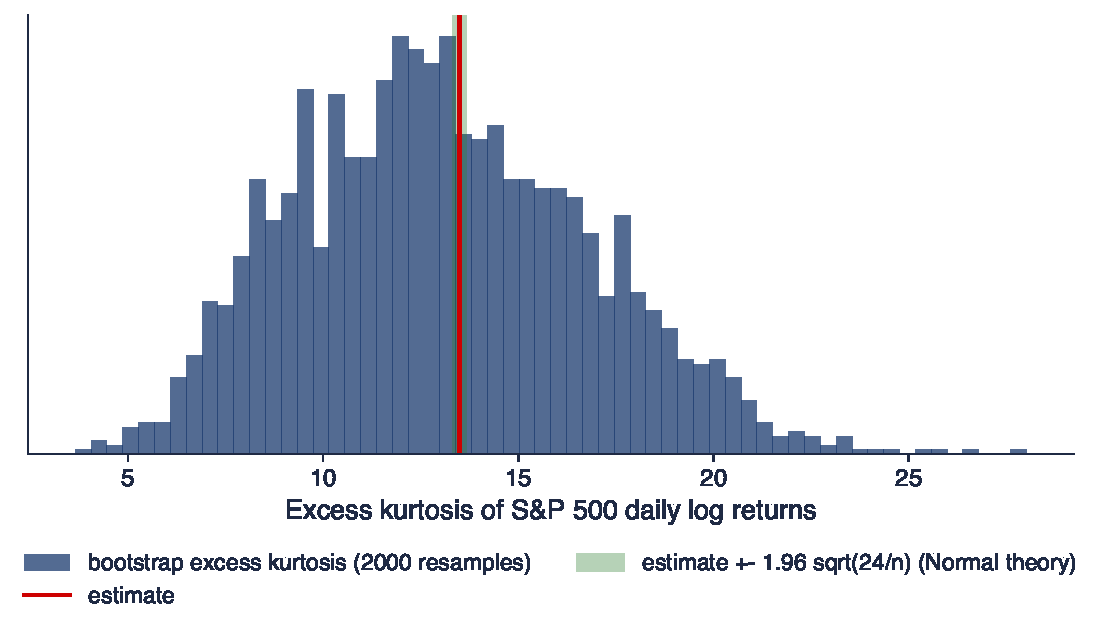
\includegraphics[width=1.0\textwidth,height=0.55\textheight,keepaspectratio]{ch2_sem_b1.pdf}
\end{center}
\vspace{-2mm}

\end{column}
\begin{column}{0.50\textwidth}
\begin{itemize}
    \item $n = 4\,201$; media $0{,}045\%$, abaterea std. $1{,}08\%$; cea mai proastă zi $-12{,}8\%$, pe 16 martie 2020
    \item $S = -0{,}61$ (SE $0{,}038$), $K = 13{,}49$ (SE $0{,}076$); $\text{JB} = 32\,113$: normalitatea respinsă
    \item Teoria Normală: $K \in [13{,}34; 13{,}64]$; bootstrap: $[6{,}7; 20{,}6]$; pentru $S$, bootstrap $[-1{,}54; 0{,}29]$
    \item Interpretare: $\sqrt{24/n}$ presupune date Normale; cu cozi groase, $K$ depinde de cîteva zile, iar prezența lor în reeșantionare îl mută mult; abaterea standard bootstrap a lui $K$ este de 50 de ori mai mare
    \item Intervalul asimetriei conține 0: semnul lui $S$ nu este sigur
\end{itemize}
\end{column}
\end{columns}\sfmquantlet{Ch_02}{SFM_ch2_seminar}
\end{frame}

\begin{frame}{B2: încă trei serii [Propus]}
\itemsize{\footnotesize}
\begin{itemize}
\item \textbf{Întrebarea}: care dintre BET, Bitcoin și OMV Petrom este cel mai departe de distribuția Normală și cît contează o singură zi?
\item \textbf{Date}: randamente logaritmice zilnice, 2010--2026 (Bitcoin din 2014), fiecare pe calendarul ei; model: B1
\item \textbf{Cerințe}
\begin{enumerate}
    \item Calculați $n$, media, abaterea standard, $S$, $K$ și JB pentru fiecare serie.
    \item Eliminați cel mai mare randament în valoare absolută din fiecare serie și recalculați $K$.
    \item Interpretare: ce vă spune schimbarea lui $K$ despre aplatizare ca rezumat al riscului?
\end{enumerate}
\item \textbf{Raportați}: un tabel și două fraze
\item Notebook: secțiunea B2
\end{itemize}
\end{frame}

\ifsolutions
\begin{frame}{B2: rezolvare [Propus]}
\itemsize{\footnotesize}
\begin{center}
\footnotesize
\begin{tabular}{lrrrrrrr}
\toprule
Seria & $n$ & Media & Ab. std. & $S$ & $K$ & JB & $K$ fără max \\
\midrule
BET & 4\,186 & $0{,}046$ & $1{,}07$ & $-0{,}98$ & $17{,}9$ & 56\,762 & $15{,}3$ \\
Bitcoin & 4\,384 & $0{,}118$ & $3{,}49$ & $-0{,}70$ & $12{,}0$ & 26\,482 & $5{,}3$ \\
OMV Petrom & 3\,815 & $0{,}076$ & $1{,}62$ & $-0{,}54$ & $8{,}9$ & 12\,832 & $7{,}0$ \\
\bottomrule
\end{tabular}
\end{center}
\begin{itemize}
    \item Zilele eliminate: BET 19 decembrie 2018 ($-11{,}9\%$), Bitcoin 12 martie 2020 ($-46{,}5\%$), SNP 25 mai 2010 ($-15{,}8\%$)
    \item Cel mai departe de distribuția Normală după $K$ și JB: BET; toate trei respinse
    \item Interpretare: o zi din mii mută aplatizarea Bitcoin de la 12{,}0 la 5{,}3; $K$ este un rezumat fragil, raportați-l împreună cu extremele
\end{itemize}\sfmquantlet{Ch_02}{SFM_ch2_seminar}
\end{frame}
\fi

\begin{frame}{B3: distribuția Normală sau Student-$t$ pentru BET? [Rezolvat]}
\itemsize{\footnotesize}
\begin{itemize}
\item \textbf{Întrebarea}: descrie o distribuție Student-$t$ randamentele zilnice ale BET mai bine decît distribuția Normală și unde greșește fiecare?
\item \textbf{Date}: închiderile BET, 2010--2026, randamente logaritmice zilnice în \%
\item \textbf{Cerințe}
\begin{enumerate}
    \item Desenați QQ plot-ul randamentelor standardizate față de $N(0,1)$.
    \item Estimați o distribuție Student-$t$ prin verosimilitate maximă și desenați QQ plot-ul față de $t$ estimată.
    \item Comparați log-verosimilitățile și AIC ale celor două modele.
    \item Interpretare: unde greșește distribuția Normală și unde greșește $t$ estimată?
\end{enumerate}
\item \textbf{Raportați}: $\hat\nu$, $\hat m$, $\hat s$, două valori AIC, două QQ plots, o frază
\item Notebook: secțiunea B3
\end{itemize}
\end{frame}

\begin{frame}{B3: rezolvare [Rezolvat]}
\itemsize{\scriptsize}
\begin{columns}[T]
\begin{column}{0.50\textwidth}
\begin{center}
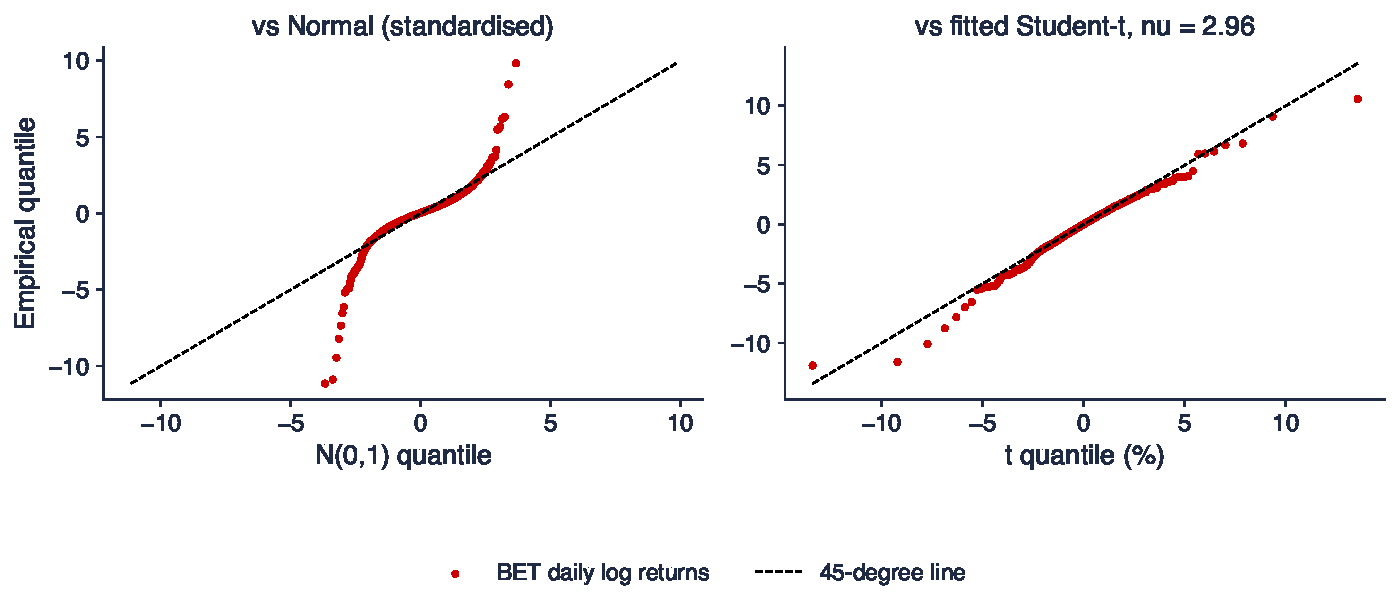
\includegraphics[width=1.0\textwidth,height=0.55\textheight,keepaspectratio]{ch2_sem_b3.pdf}
\end{center}
\vspace{-2mm}

\end{column}
\begin{column}{0.48\textwidth}
\begin{itemize}
    \item $\hat\nu = 2{,}96$, $\hat m = 0{,}078\%$, $\hat s = 0{,}628\%$; abaterea std. implicată $\hat s\sqrt{\hat\nu/(\hat\nu - 2)} = 1{,}10\%$
    \item $\ell_t = -5496$ față de $\ell_N = -6224$; $\text{AIC}_N - \text{AIC}_t = 1454$: $t$ cîștigă clar
    \item Cel mai mic randament $-11{,}9\%$; cuantila corespunzătoare: distribuția Normală $-3{,}9\%$, $t$ estimată $-13{,}4\%$
    \item Interpretare: distribuția Normală ratează ambele cozi (forma de S); $t$ se potrivește centrului și majorității cozilor, dar cuantilele ei extreme trec puțin dincolo de date
\end{itemize}
\end{column}
\end{columns}\sfmquantlet{Ch_02}{SFM_ch2_seminar}
\end{frame}

\begin{frame}{B4: cîte zile de 4 sigma? [Propus]}
\itemsize{\footnotesize}
\begin{itemize}
\item \textbf{Întrebarea}: cîte zile de 4 sigma au S\&P 500, DAX, BET și Bitcoin și ce model dă numărul corect?
\item \textbf{Date}: randamente logaritmice zilnice, 2010--2026 (Bitcoin din 2014); model: B3
\item \textbf{Cerințe}
\begin{enumerate}
    \item Numărați zilele cu $|r_t - \bar r| > 4s$ din fiecare serie.
    \item Calculați numărul așteptat în distribuția Normală și probabilitatea Poisson de a vedea cel puțin numărul observat.
    \item Calculați numărul așteptat cu distribuția Student-$t$ estimată (același prag $\bar r \pm 4s$).
    \item Interpretare: este distribuția Student-$t$ prea grea, prea ușoară sau potrivită pentru fiecare serie?
\end{enumerate}
\item \textbf{Raportați}: un tabel și o frază pentru fiecare serie
\item Notebook: secțiunea B4
\end{itemize}
\end{frame}

\ifsolutions
\begin{frame}{B4: rezolvare [Propus]}
\itemsize{\footnotesize}
\begin{center}
\footnotesize
\begin{tabular}{lrrrrrr}
\toprule
Seria & $n$ & observate & Normal & $p$ (Poisson) & $\hat\nu$ & Student-$t$ \\
\midrule
S\&P 500 & 4\,201 & 28 & $0{,}27$ & ${2 \times 10^{-46}}$ & $2{,}78$ & $34{,}9$ \\
DAX & 4\,244 & 20 & $0{,}27$ & ${1 \times 10^{-30}}$ & $3{,}31$ & $29{,}5$ \\
BET & 4\,186 & 28 & $0{,}27$ & ${2 \times 10^{-46}}$ & $2{,}96$ & $28{,}1$ \\
Bitcoin & 4\,384 & 29 & $0{,}28$ & ${6 \times 10^{-48}}$ & $2{,}23$ & $54{,}8$ \\
\bottomrule
\end{tabular}
\end{center}
\begin{itemize}
    \item Distribuția Normală este respinsă pentru toate seriile: numerele observate sînt de 74--106 ori mai mari decît cele așteptate
    \item Interpretare: $t$ este potrivită pentru BET, ceva prea grea pentru S\&P 500 și DAX și mult prea grea pentru Bitcoin ($\hat\nu$ aproape de 2)
    \item Un singur $\nu$ ajustează întreaga distribuție prin verosimilitate, dominată de multele zile obișnuite, nu de puținele zile extreme
\end{itemize}\sfmquantlet{Ch_02}{SFM_ch2_seminar}
\end{frame}
\fi

\begin{frame}{B5: devine S\&P 500 Normal pe orizonturi mai lungi? [Rezolvat]}
\itemsize{\footnotesize}
\begin{itemize}
\item \textbf{Întrebarea}: sînt randamentele pe 5 și pe 21 de zile ale S\&P 500 mai apropiate de distribuția Normală decît cele zilnice?
\item \textbf{Date}: randamentele logaritmice zilnice ale S\&P 500, 2010--2026; randamentele pe $h$ zile sînt sume pe blocuri de $h$ zile care nu se suprapun
\item \textbf{Cerințe}
\begin{enumerate}
    \item Construiți randamentele logaritmice pe 5 și pe 21 de zile.
    \item Calculați $n$, $S$, $K$, eroarea standard $\sqrt{24/n}$ și JB cu valoarea $p$ pentru $h = 1, 5, 21$.
    \item Desenați cele trei QQ plots față de $N(0,1)$.
    \item Interpretare: este distribuția lunară Normală și de ce are testul mai puțină putere la $h = 21$?
\end{enumerate}
\item \textbf{Raportați}: un tabel cu trei rînduri, trei QQ plots, două fraze
\item Notebook: secțiunea B5
\end{itemize}
\end{frame}

\begin{frame}{B5: rezolvare [Rezolvat]}
\itemsize{\scriptsize}
\begin{center}
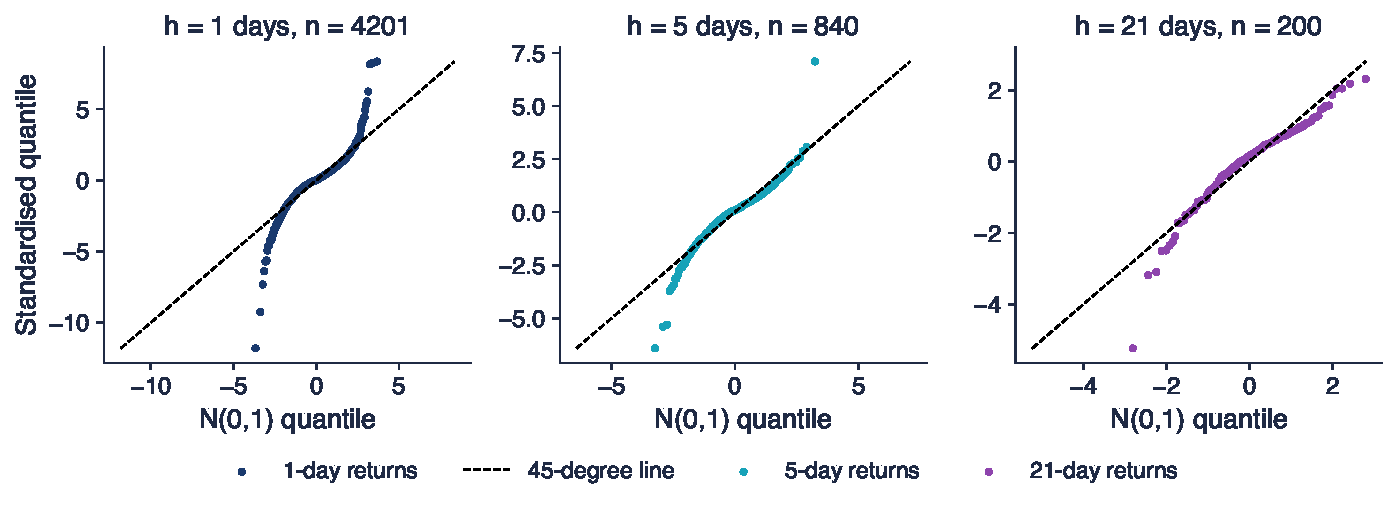
\includegraphics[width=0.96\textwidth,height=0.42\textheight,keepaspectratio]{ch2_sem_b5.pdf}
\end{center}
\vspace{-2mm}
\begin{center}
\scriptsize
\begin{tabular}{rrrrrr}
\toprule
$h$ & $n$ & $S$ & $K$ & $\sqrt{24/n}$ & JB ($p$) \\
\midrule
1 & 4201 & $-0{,}61$ & $13{,}49$ & $0{,}08$ & 32\,113 (${\approx 0}$) \\
5 & 840 & $-0{,}62$ & $7{,}06$ & $0{,}17$ & 1\,797 (${\approx 0}$) \\
21 & 200 & $-1{,}18$ & $3{,}68$ & $0{,}35$ & 159 (${2{,}9 \times 10^{-35}}$) \\
\bottomrule
\end{tabular}
\end{center}
\begin{itemize}
    \item Interpretare: $K$ scade de la 13{,}49 la 3{,}68, dar randamentele lunare tot nu sînt Normale (asimetria $-1{,}18$, martie 2020); cu doar 200 de luni, eroarea standard a lui $K$ este 0{,}35, deci abaterile mai mici n-ar fi detectate
\end{itemize}\sfmquantlet{Ch_02}{SFM_ch2_seminar}
\end{frame}

\begin{frame}{B6: sînt independente randamentele BET? [Propus]}
\itemsize{\footnotesize}
\begin{itemize}
\item \textbf{Întrebarea}: sînt randamentele zilnice ale BET necorelate și sînt ele independente?
\item \textbf{Date}: randamentele logaritmice zilnice ale BET, 2010--2026; model: B5
\item \textbf{Cerințe}
\begin{enumerate}
    \item Calculați ACF pentru $r_t$ și pentru $|r_t|$ la decalajele 1--10 și banda $\pm 1{,}96/\sqrt n$.
    \item Calculați statistica Ljung--Box $Q(10)$ pentru $r_t$ și pentru $|r_t|$ și comparați cu $\chi^2_{0{,}95}(10)$.
    \item Interpretare: pot fi randamentele necorelate, dar nu independente?
\end{enumerate}
\item \textbf{Raportați}: două coloane ACF, două valori $Q$, o frază
\item Notebook: secțiunea B6
\end{itemize}
\end{frame}

\ifsolutions
\begin{frame}{B6: rezolvare [Propus]}
\itemsize{\footnotesize}
\begin{itemize}
    \item $n = 4\,186$, banda $\pm 0{,}030$
    \item $r_t$: $\hat\rho(1), \hat\rho(2), \hat\rho(3) = 0{,}034; 0{,}056; -0{,}018$; 5 din 10 decalaje în afara benzii; $Q(10) = 45{,}7$ ($p = 1{,}6 \times 10^{-6}$)
    \item $|r_t|$: $0{,}335; 0{,}241; 0{,}260$, \dots, $0{,}201$ la decalajul 10; $Q(10) = 2120$, mult peste $18{,}31$
    \item Testul pentru $r_t$ respinge și el, dar autocorelațiile sînt cel mult 0{,}06 în valoare absolută, iar banda presupune date i.i.d., ceea ce volatility clustering încalcă
    \item Interpretare: da; independența ar face și $|r_t|$ necorelate; autocorelația puternică a lui $|r_t|$ arată că mărimea randamentelor este previzibilă, semnul lor mult mai puțin
\end{itemize}\sfmquantlet{Ch_02}{SFM_ch2_seminar}
\end{frame}
\fi

\begin{frame}{B7: seamănă Bitcoin cu un indice bursier? [Propus]}
\itemsize{\footnotesize}
\begin{itemize}
\item \textbf{Întrebarea}: arată atît S\&P 500, cît și Bitcoin efectul de levier și asimetria cîștig/pierdere?
\item \textbf{Date}: randamente logaritmice zilnice, S\&P 500 2010--2026, Bitcoin 2014--2026; model: B5
\item \textbf{Cerințe}
\begin{enumerate}
    \item Calculați $L(k) = \text{Corr}(r_t, |r_{t+k}|)$ pentru $k = 1, \dots, 5$ și media lor, cu banda $\pm 1{,}96/\sqrt n$.
    \item Numărați zilele sub $\bar r - 4s$ și peste $\bar r + 4s$; testați dacă scăderile și creșterile sînt la fel de probabile (testul binomial, $p = 0{,}5$).
    \item Comparați $|q_{0{,}01}|$ cu $q_{0{,}99}$ și asimetria.
    \item Interpretare: ce fapte stilizate ale indicilor bursieri are și Bitcoin?
\end{enumerate}
\item \textbf{Raportați}: un tabel și două fraze
\item Notebook: secțiunea B7
\end{itemize}
\end{frame}

\ifsolutions
\begin{frame}{B7: rezolvare [Propus]}
\itemsize{\footnotesize}
\begin{center}
\footnotesize
\begin{tabular}{lrrrrrrrr}
\toprule
Seria & $L(1)$ & $\bar L(1..5)$ & banda & $< -4s$ & $> +4s$ & $p$ & $|q_{0{,}01}|$ & $q_{0{,}99}$ \\
\midrule
S\&P 500 & $-0{,}122$ & $-0{,}121$ & $0{,}030$ & 16 & 12 & $0{,}57$ & $3{,}15$ & $2{,}61$ \\
Bitcoin & $-0{,}073$ & $-0{,}031$ & $0{,}030$ & 18 & 11 & $0{,}26$ & $10{,}51$ & $9{,}87$ \\
\bottomrule
\end{tabular}
\end{center}
\begin{itemize}
    \item Levier: clar pentru S\&P 500 ($\bar L = -0{,}121$, de 4 ori banda); pentru Bitcoin doar la decalajul 1, media este la marginea benzii
    \item Mai multe căderi extreme decît creșteri la ambele, dar cu atît de puține zile extreme testul binomial nu poate respinge egalitatea ($p = 0{,}57$ și $0{,}26$)
    \item Interpretare: Bitcoin are cozi groase, clustering și asimetrie negativă ($-0{,}70$), dar efectul de levier este slab: în spatele lui nu există o firmă cu datorii
\end{itemize}\sfmquantlet{Ch_02}{SFM_ch2_seminar}
\end{frame}
\fi


%=============================================================================
\section{Partea C: întrebări deschise și critica unui răspuns AI}
%=============================================================================

\begin{frame}{C1: devin mai subțiri cozile Bitcoin? [Propus]}
\itemsize{\footnotesize}
\begin{itemize}
\item \textbf{Întrebarea}: a devenit mai subțire coada randamentelor zilnice ale Bitcoin din 2015, pe măsură ce piața s-a maturizat?
\item \textbf{Date}: randamentele logaritmice zilnice ale Bitcoin și S\&P 500, 2015--2026; modele: B3, B5
\item \textbf{Cerințe}
\begin{enumerate}
    \item Estimați o distribuție Student-$t$ și calculați excesul de aplatizare pentru fiecare an calendaristic și fiecare serie.
    \item Calculați corelația rangurilor Spearman între an și $\hat\nu$.
    \item Estimați o distribuție $t$ pe 2015--2020 și una pe 2021--2026 și comparați $\hat\nu$.
    \item Propuneți o cale de a face răspunsul mai sigur (intervale, alte ferestre, alte active cripto).
    \item Interpretare: ce ne pot spune 12 estimări anuale despre un trend?
\end{enumerate}
\item \textbf{Raportați}: un tabel, corelația rangurilor cu valoarea $p$, un scurt plan de proiect
\item Notebook: secțiunea C1
\end{itemize}
\end{frame}

\ifsolutions
\begin{frame}{C1: analiză de referință [Propus]}
\itemsize{\footnotesize}
\begin{itemize}
    \item Bitcoin: $\hat\nu$ anual între 1{,}5 și 5{,}1; Spearman cu anul $0{,}63$ ($p = 0{,}03$, 12 ani)
    \item Două jumătăți: $\hat\nu$ = 1{,}91 (2015--2020) și 2{,}69 (2021--2026)
    \item S\&P 500: Spearman $0{,}31$ ($p = 0{,}32$); $\hat\nu$ = 2{,}13 și 4{,}06: și reperul s-a schimbat
    \item Dovezi slabe de cozi mai subțiri pentru Bitcoin, dar un singur test pe 12 puncte zgomotoase, ales după ce am văzut datele; doar anii calmi pot crește $\hat\nu$
    \item Direcții de proiect: ferestre mobile cu intervale bootstrap, randamente împărțite la o volatilitate mobilă, Ethereum și Solana, estimatorul Hill din \sfmchlink{https://danpele.github.io/SFM/RO/Cursuri/capitol5_cozi_groase_evt.pdf}{Capitolul 5}
\end{itemize}\sfmquantlet{Ch_02}{SFM_ch2_seminar}
\end{frame}
\fi

\begin{frame}{C2: verificați un răspuns AI [Propus]}
\itemsize{\scriptsize}
\begin{itemize}
    \item Un student a întrebat un asistent AI: „Descrie distribuția randamentelor zilnice ale S\&P 500 în 2010--2026.” Răspunsul:
    \item \aiprompt{(a) Excesul de aplatizare este 13{,}5; cum distribuția Normală are aplatizarea 0, aplatizarea S\&P 500 este 13{,}5.}
    \item \aiprompt{(b) JB = 32\,113 cu p = 0,000, ceea ce dovedește că randamentele urmează o distribuție Student-t.}
    \item \aiprompt{(c) O zi Normală de 4 sigma apare o dată la 15\,787 de zile; cele 28 de zile de acest fel din 4\,201 sînt doar ghinion.}
    \item \aiprompt{(d) Autocorelația la decalajul 1 este doar -0{,}11, deci randamentele sînt independente și volatilitatea nu poate fi prevăzută.}
    \item \aiprompt{(e) Cu randamente logaritmice anuale N(7\%, 18\%\textasciicircum 2), valoarea așteptată a 100 investiți după un an este 100 exp(0,07) = 107{,}25.}
    \item Cerințe
    \begin{itemize}
        \item 1. Pentru fiecare afirmație spuneți dacă este corectă; dacă nu, dați afirmația corectă și cifra corectă din notebook (secțiunea C2).
        \item 2. Raportați: o listă de cinci verdicte, fiecare cu un rînd de justificare.
    \end{itemize}
\end{itemize}
\end{frame}

\ifsolutions
\begin{frame}{C2: rezolvare [Propus]}
\itemsize{\footnotesize}
\begin{itemize}
    \item (a) Greșit: aplatizarea Normală este 3 (excesul 0); aplatizarea $= 13{,}5 + 3 = 16{,}5$
    \item (b) Greșit: JB doar respinge normalitatea; $t$ estimată ($\hat\nu = 2{,}78$) este mai bună după AIC, dar QQ plot-ul ei tot ratează extremele și este simetrică
    \item (c) Greșit: așteptarea Normală este de $0{,}27$ zile; a vedea 28 are probabilitatea Poisson de circa $2 \times 10^{-46}$: greșit este modelul, nu norocul
    \item (d) Greșit: necorelat nu înseamnă independent; ACF a lui $|r_t|$ este $0{,}31$ la decalajul 1 și $0{,}26$ la decalajul 10, Ljung--Box $Q(10) = 3859$: volatilitatea este previzibilă
    \item (e) Greșit: $100e^{0{,}07} = 107{,}25$ este mediana; media este $100e^{0{,}07 + 0{,}18^2/2} = 109{,}00$
\end{itemize}\sfmquantlet{Ch_02}{SFM_ch2_seminar}
\end{frame}
\fi


%=============================================================================
\section{Încheiere}
%=============================================================================

\begin{frame}{Ce rămîne de azi}
\itemsize{\small}
\begin{itemize}
    \item Distribuția Normală face zilele de 4 sigma aproape imposibile; piețele reale le au la cîteva luni
    \item Prețuri lognormale: mediana este sub medie cu volatility drag
    \item Asimetria și aplatizarea sînt fragile: raportați intervale bootstrap și extremele
    \item Distribuția Student-$t$ se potrivește mult mai bine decît distribuția Normală, dar nu perfect
    \item Randamentele sînt aproape necorelate, dar nu independente: mărimea lor este previzibilă
    \item Un răspuns AI este o ciornă: verificați fiecare definiție, model și cifră
\end{itemize}
\end{frame}

\begin{frame}{După seminar}
\itemsize{\small}
\begin{itemize}
    \item Cursul 2 dezvoltă fiecare temă de azi: modelele Normal și lognormal, CLT, momente și teste, distribuția Student-$t$ și șase fapte stilizate
    \item Încercați cerințele [Propus] în notebook; rezolvările se discută la seminar
    \item C1 poate deveni un proiect de echipă: ferestre mobile, intervale bootstrap, mai multe active cripto
    \item Lectură: \refFHH, secț.~3.3 și secț.~11.2; exerciții rezolvate: \refFHHex
\end{itemize}
\end{frame}


%=============================================================================
\section{Bibliografie}
%=============================================================================

\begin{frame}{Bibliografie}
\itemsize{\tiny}
\begin{itemize}
    \item Borak, S., Härdle, W.K., López-Cabrera, B. (2013). \href{https://doi.org/10.1007/978-3-642-33929-5}{\textit{Statistics of Financial Markets: Exercises and Solutions}}, 2nd ed. Springer.
    \item Cont, R. (2001). \href{https://doi.org/10.1080/713665670}{Empirical properties of asset returns: stylized facts and statistical issues}. \textit{Quantitative Finance}, 1(2), 223--236.
    \item Franke, J., Härdle, W.K., Hafner, C.M. (2019). \href{https://doi.org/10.1007/978-3-030-13751-9}{\textit{Statistics of Financial Markets: An Introduction}}, 5th ed. Springer.
    \item Jarque, C.M., Bera, A.K. (1987). \href{https://doi.org/10.2307/1403192}{A test for normality of observations and regression residuals}. \textit{International Statistical Review}, 55(2), 163--172.
    \item Ljung, G.M., Box, G.E.P. (1978). \href{https://doi.org/10.1093/biomet/65.2.297}{On a measure of lack of fit in time series models}. \textit{Biometrika}, 65(2), 297--303.
    \item Student (1908). \href{https://doi.org/10.1093/biomet/6.1.1}{The probable error of a mean}. \textit{Biometrika}, 6(1), 1--25.
\end{itemize}
\end{frame}

\end{document}
